\documentclass[12pt,a4paper]{article}

% ── Packages ─────────────────────────────────────────────────────────────
\usepackage[margin=2.5cm]{geometry}
\usepackage{graphicx}
\usepackage{booktabs}
\usepackage{longtable}
\usepackage{array}
\usepackage{hyperref}
\usepackage{xcolor}
\usepackage{caption}
\usepackage{subcaption}
\usepackage{float}
\usepackage{listings}
\usepackage{titlesec}
\usepackage{parskip}
\usepackage{fancyhdr}
\usepackage{enumitem}
\usepackage{amsmath}
\usepackage{multirow}
\usepackage[T1]{fontenc}
\usepackage{lmodern}

% ── Colours ──────────────────────────────────────────────────────────────
\definecolor{headerblue}{RGB}{31,73,125}
\definecolor{lightgray}{RGB}{230,230,230}
\definecolor{codegray}{RGB}{245,245,245}
\definecolor{keywordred}{RGB}{180,0,0}

% ── Section formatting ───────────────────────────────────────────────────
\titleformat{\section}{\large\bfseries\color{headerblue}}{}{0em}{\thesection\quad}[\titlerule]
\titleformat{\subsection}{\normalsize\bfseries\color{headerblue}}{}{0em}{\thesubsection\quad}
\titleformat{\subsubsection}{\normalsize\bfseries}{}{0em}{\thesubsubsection\quad}

% ── Code listing style ───────────────────────────────────────────────────
\lstset{
  backgroundcolor=\color{codegray},
  basicstyle=\ttfamily\small,
  breaklines=true,
  frame=single,
  rulecolor=\color{gray},
  keywordstyle=\color{keywordred}\bfseries,
  commentstyle=\color{gray},
  stringstyle=\color{blue},
  showstringspaces=false,
  tabsize=4
}

% ── Header / Footer ──────────────────────────────────────────────────────
\pagestyle{fancy}
\fancyhf{}
\fancyhead[L]{\small India Cost of Living Index}
\fancyhead[R]{\small BMP Data Modelling}
\fancyfoot[C]{\thepage}
\renewcommand{\headrulewidth}{0.4pt}

% ── Hyperref ─────────────────────────────────────────────────────────────
\hypersetup{
  colorlinks=true,
  linkcolor=headerblue,
  urlcolor=headerblue,
  citecolor=headerblue,
  pdftitle={India Cost of Living Index -- Project Report},
  pdfauthor={BMP Data Modelling}
}

% ─────────────────────────────────────────────────────────────────────────
\begin{document}

% ── Title page ───────────────────────────────────────────────────────────
\begin{titlepage}
  \centering
  \vspace*{2cm}
  {\Huge\bfseries\color{headerblue} India Cost of Living Index\\[0.4cm]}
  {\Large\bfseries Comprehensive Analysis of 50 Indian Cities\\[0.8cm]}
  \rule{\linewidth}{0.5pt}\\[0.6cm]
  {\large Project Report}\\[0.4cm]
  {\large BMP Data Modelling}\\[0.4cm]
  {\large April 2026}\\[1cm]
  \rule{\linewidth}{0.5pt}
  \vfill
  \begin{tabular}{ll}
    \textbf{Status:}   & Complete \\
    \textbf{Language:} & Python 3.8+ \\
    \textbf{Cities:}   & 50 Indian Cities \\
    \textbf{Data Files:} & 94+ raw files \\
    \textbf{Base City:} & Delhi (Index = 100) \\
  \end{tabular}
\end{titlepage}

\tableofcontents
\newpage

% ─────────────────────────────────────────────────────────────────────────
\section{Executive Summary}

This project delivers a \textbf{data-driven Cost of Living Index} for 50 major Indian cities,
built from over 94 raw data files sourced from real-world platforms (MagicBricks, Blinkit,
Uber, Swiggy, and more). The index uses an expenditure-weighted formula with Delhi anchored
at 100 to compare the true cost of everyday life across India.

\textbf{Key Finding:} Mumbai is 62.8\% more expensive than Delhi. The most affordable city,
Malappuram, scores 69.54 -- nearly 43\% less expensive than Mumbai.

\subsection{Top 5 Most Expensive Cities}

\begin{table}[H]
  \centering
  \begin{tabular}{clc}
    \toprule
    \textbf{Rank} & \textbf{City} & \textbf{Index} \\
    \midrule
    1 & Mumbai      & 162.79 \\
    2 & Bengaluru   & 114.76 \\
    3 & Kozhikode   & 107.66 \\
    4 & Hyderabad   & 107.09 \\
    5 & Patna       & 100.72 \\
    \bottomrule
  \end{tabular}
  \caption{Top 5 most expensive cities (Delhi = 100)}
\end{table}

\subsection{Top 5 Most Affordable Cities}

\begin{table}[H]
  \centering
  \begin{tabular}{clc}
    \toprule
    \textbf{Rank} & \textbf{City} & \textbf{Index} \\
    \midrule
    1 & Malappuram      & 69.54 \\
    2 & Solapur         & 68.20 \\
    3 & Tiruchirappalli & 71.41 \\
    4 & Ludhiana        & 72.50 \\
    5 & Jamnagar        & 72.77 \\
    \bottomrule
  \end{tabular}
  \caption{Top 5 most affordable cities (Delhi = 100)}
\end{table}

% ─────────────────────────────────────────────────────────────────────────
\section{Data Sources and Files Used}

\subsection{Housing Data -- MagicBricks}

\begin{itemize}[leftmargin=*]
  \item \textbf{Location:} \texttt{data/raw/Magic Bricks data/}
  \item \textbf{Format:} CSV \quad \textbf{Files:} 50 (one per city)
  \item \textbf{Key columns:} \texttt{city\_name}, \texttt{carpet\_area}, \texttt{price}, \texttt{price\_per\_sq\_ft}
  \item \textbf{Coverage:} 50/50 cities (100\%) \quad \textbf{Listings per city:} 100--500
\end{itemize}

Property listing files scraped from MagicBricks for every major Indian city. The metric used
is the \textbf{IQR-cleaned median price per sq ft} -- robust to luxury outliers.

\begin{table}[H]
  \centering
  \begin{tabular}{lc}
    \toprule
    \textbf{City} & \textbf{Price/sq ft (INR)} \\
    \midrule
    Delhi      & 10,231 \\
    Mumbai     & 23,619 \\
    Bengaluru  & 11,029 \\
    Malappuram &  1,512 \\
    \bottomrule
  \end{tabular}
  \caption{Sample housing prices}
\end{table}

% ──────────────────────────────────────────────────────────────
\subsection{Grocery Data -- Blinkit}

\begin{itemize}[leftmargin=*]
  \item \textbf{Location:} \texttt{data/raw/grocery/blinkit\_citywise/}
  \item \textbf{Format:} Excel (.xlsx) \quad \textbf{Files:} 41
  \item \textbf{Columns:} Product name | Price (INR)
  \item \textbf{Coverage:} 41/50 cities (82\%) -- 9 missing cities filled with median (INR 42)
  \item \textbf{Products per city:} 50--200 items
\end{itemize}

City-specific grocery price lists from Blinkit (online delivery). Covers staples: rice, wheat,
vegetables, dairy, and packaged goods.

\begin{table}[H]
  \centering
  \begin{tabular}{lc}
    \toprule
    \textbf{City} & \textbf{Median Grocery Price (INR)} \\
    \midrule
    Delhi     & 42.00 \\
    Mumbai    & 49.50 \\
    Kozhikode & 56.00 \\
    Nashik    & 36.00 \\
    \bottomrule
  \end{tabular}
  \caption{Sample median grocery prices}
\end{table}

% ──────────────────────────────────────────────────────────────
\subsection{Transport Data}

\begin{itemize}[leftmargin=*]
  \item \textbf{Uber prices:} \texttt{City Wise Uber Price Per km .xlsx} (42 cities)
  \item \textbf{Fuel prices:} \texttt{Fuel Prices by city (1).csv} (50 cities -- petrol, diesel, CNG, LPG)
\end{itemize}

Uber per-km price is the \textbf{primary transport metric} used in the index. Price range:
INR 10.61 -- 48.37 per km.

\begin{table}[H]
  \centering
  \begin{tabular}{lcc}
    \toprule
    \textbf{City} & \textbf{Uber (INR/km)} & \textbf{Avg Fuel (INR/L)} \\
    \midrule
    Delhi     & 20.00 & 91.26 \\
    Mumbai    & 44.07 & 96.75 \\
    Bengaluru & 43.26 & 96.94 \\
    \bottomrule
  \end{tabular}
  \caption{Sample transport prices}
\end{table}

% ──────────────────────────────────────────────────────────────
\subsection{Healthcare Data}

\begin{itemize}[leftmargin=*]
  \item \textbf{File:} \texttt{General Physician Fee City wise.xlsx}
  \item \textbf{Format:} Wide -- multiple doctor fee samples per city across columns
  \item \textbf{Coverage:} 50/50 cities \quad \textbf{Samples per city:} 10--30
\end{itemize}

Median general physician consultation fee used after IQR outlier removal (removes specialist
and premium clinic fees).

% ──────────────────────────────────────────────────────────────
\subsection{Education Data -- Tutor Marketplace}

\begin{itemize}[leftmargin=*]
  \item \textbf{File:} \texttt{TutorData\_Filtered.xlsx}
  \item \textbf{Total records:} 60,256 listings; \textbf{after per-hour filter:} 46,965
  \item \textbf{Fee format:} Range strings -- ``INR 300--1000/hour'' parsed with regex
  \item \textbf{Aggregation:} Mean of IQR-cleaned hourly rates
  \item \textbf{Coverage:} 50/50 cities (avg 940 listings per city)
\end{itemize}

\begin{table}[H]
  \centering
  \begin{tabular}{lc}
    \toprule
    \textbf{City} & \textbf{Avg Tutor Fee/hr (INR)} \\
    \midrule
    Delhi      & 539 \\
    Mumbai     & 614 \\
    Malappuram & 253 \\
    \bottomrule
  \end{tabular}
  \caption{Sample tutor hourly rates}
\end{table}

% ──────────────────────────────────────────────────────────────
\subsection{Utilities -- Electricity}

\begin{itemize}[leftmargin=*]
  \item \textbf{Files:} \texttt{Electricity Price.xlsx} (primary), backup copy also present
  \item \textbf{Metric:} Effective tariff rate (INR per kWh unit)
  \item \textbf{Coverage:} 50/50 cities \quad \textbf{Range:} INR 3.00--8.50/unit
\end{itemize}

% ──────────────────────────────────────────────────────────────
\subsection{Entertainment Data}

\begin{itemize}[leftmargin=*]
  \item \textbf{Movie tickets:} \texttt{Movieticketprices.xlsx} -- 5--15 theater samples per city
  \item \textbf{Restaurant prices:} \texttt{swiggy dataset.xlsx} -- 50--200 listings per city,
        ``for two'' pricing halved to per-person
\end{itemize}

\begin{table}[H]
  \centering
  \begin{tabular}{lcc}
    \toprule
    \textbf{City} & \textbf{Movie Ticket (INR)} & \textbf{Restaurant/person (INR)} \\
    \midrule
    Delhi  & 390 & 125 \\
    Mumbai & 600 & 150 \\
    Salem  &  60 & 125 \\
    \bottomrule
  \end{tabular}
  \caption{Sample entertainment prices}
\end{table}

% ─────────────────────────────────────────────────────────────────────────
\section{Data Processing Methodology}

\subsection{Outlier Removal -- IQR Method}

Applied to all multi-sample datasets (housing, grocery, healthcare, education, movies,
restaurants):

\[
  \text{IQR} = Q_3 - Q_1
\]
\[
  \text{Valid range} = \left[Q_1 - 1.5 \times \text{IQR},\; Q_3 + 1.5 \times \text{IQR}\right]
\]

This removes luxury properties, IMAX tickets, specialist doctors, and premium tutors while
preserving typical household costs.

\subsection{Component Index Calculation}

Each component index is relative to Delhi (base = 100):

\[
  \text{Component Index}_{\text{city}} = \frac{\text{City Price}}{\text{Delhi Price}} \times 100
\]

\subsection{Weighted Overall Index}

\begin{table}[H]
  \centering
  \begin{tabular}{lccc}
    \toprule
    \textbf{Component} & \textbf{Raw Weight} & \textbf{Normalised Weight} & \textbf{Justification} \\
    \midrule
    Grocery       & 0.30   & 36.36\% & Daily food -- largest expense \\
    Housing       & 0.25   & 30.30\% & Rent/EMI -- major fixed cost \\
    Transport     & 0.09   & 10.91\% & Daily commute \\
    Healthcare    & 0.053  &  6.42\% & Essential medical services \\
    Education     & 0.050  &  6.06\% & Tutor hourly rates \\
    Restaurant    & 0.040  &  4.85\% & Dining out / food delivery \\
    Electricity   & 0.025  &  3.03\% & Monthly utility bill \\
    Movies        & 0.0171 &  2.07\% & Entertainment proxy \\
    \midrule
    \textbf{Total} & \textbf{0.8251} & \textbf{100\%} & \\
    \bottomrule
  \end{tabular}
  \caption{Component weights (raw values re-normalised at runtime)}
\end{table}

\[
  \text{Cost Index} = \sum_{i} w_i \times \text{Component Index}_i
\]

\[
\begin{aligned}
  \text{Cost Index} =\; &(\text{Grocery} \times 0.3636) + (\text{Housing} \times 0.3030) \\
                      + &(\text{Transport} \times 0.1091) + (\text{Healthcare} \times 0.0642) \\
                      + &(\text{Education} \times 0.0606) + (\text{Restaurant} \times 0.0485) \\
                      + &(\text{Electricity} \times 0.0303) + (\text{Movies} \times 0.0207)
\end{aligned}
\]

\subsection{Missing Data Strategy}

Missing values are filled with the \textbf{median} across all available cities -- robust to
outliers and avoids over/underestimation.

\begin{table}[H]
  \centering
  \begin{tabular}{lcc}
    \toprule
    \textbf{Component}  & \textbf{Missing Cities} & \textbf{Fill Value} \\
    \midrule
    Uber price          & 8  & INR 18.91/km \\
    Grocery price       & 9  & INR 42.00 \\
    Housing price       & 0  & -- \\
    \bottomrule
  \end{tabular}
  \caption{Missing value imputation summary}
\end{table}

% ─────────────────────────────────────────────────────────────────────────
\section{Output Visualizations}

The project generates \textbf{23 charts} in \texttt{outputs/visualizations/}.
Key visualizations are described below.

\begin{figure}[H]
  \centering
  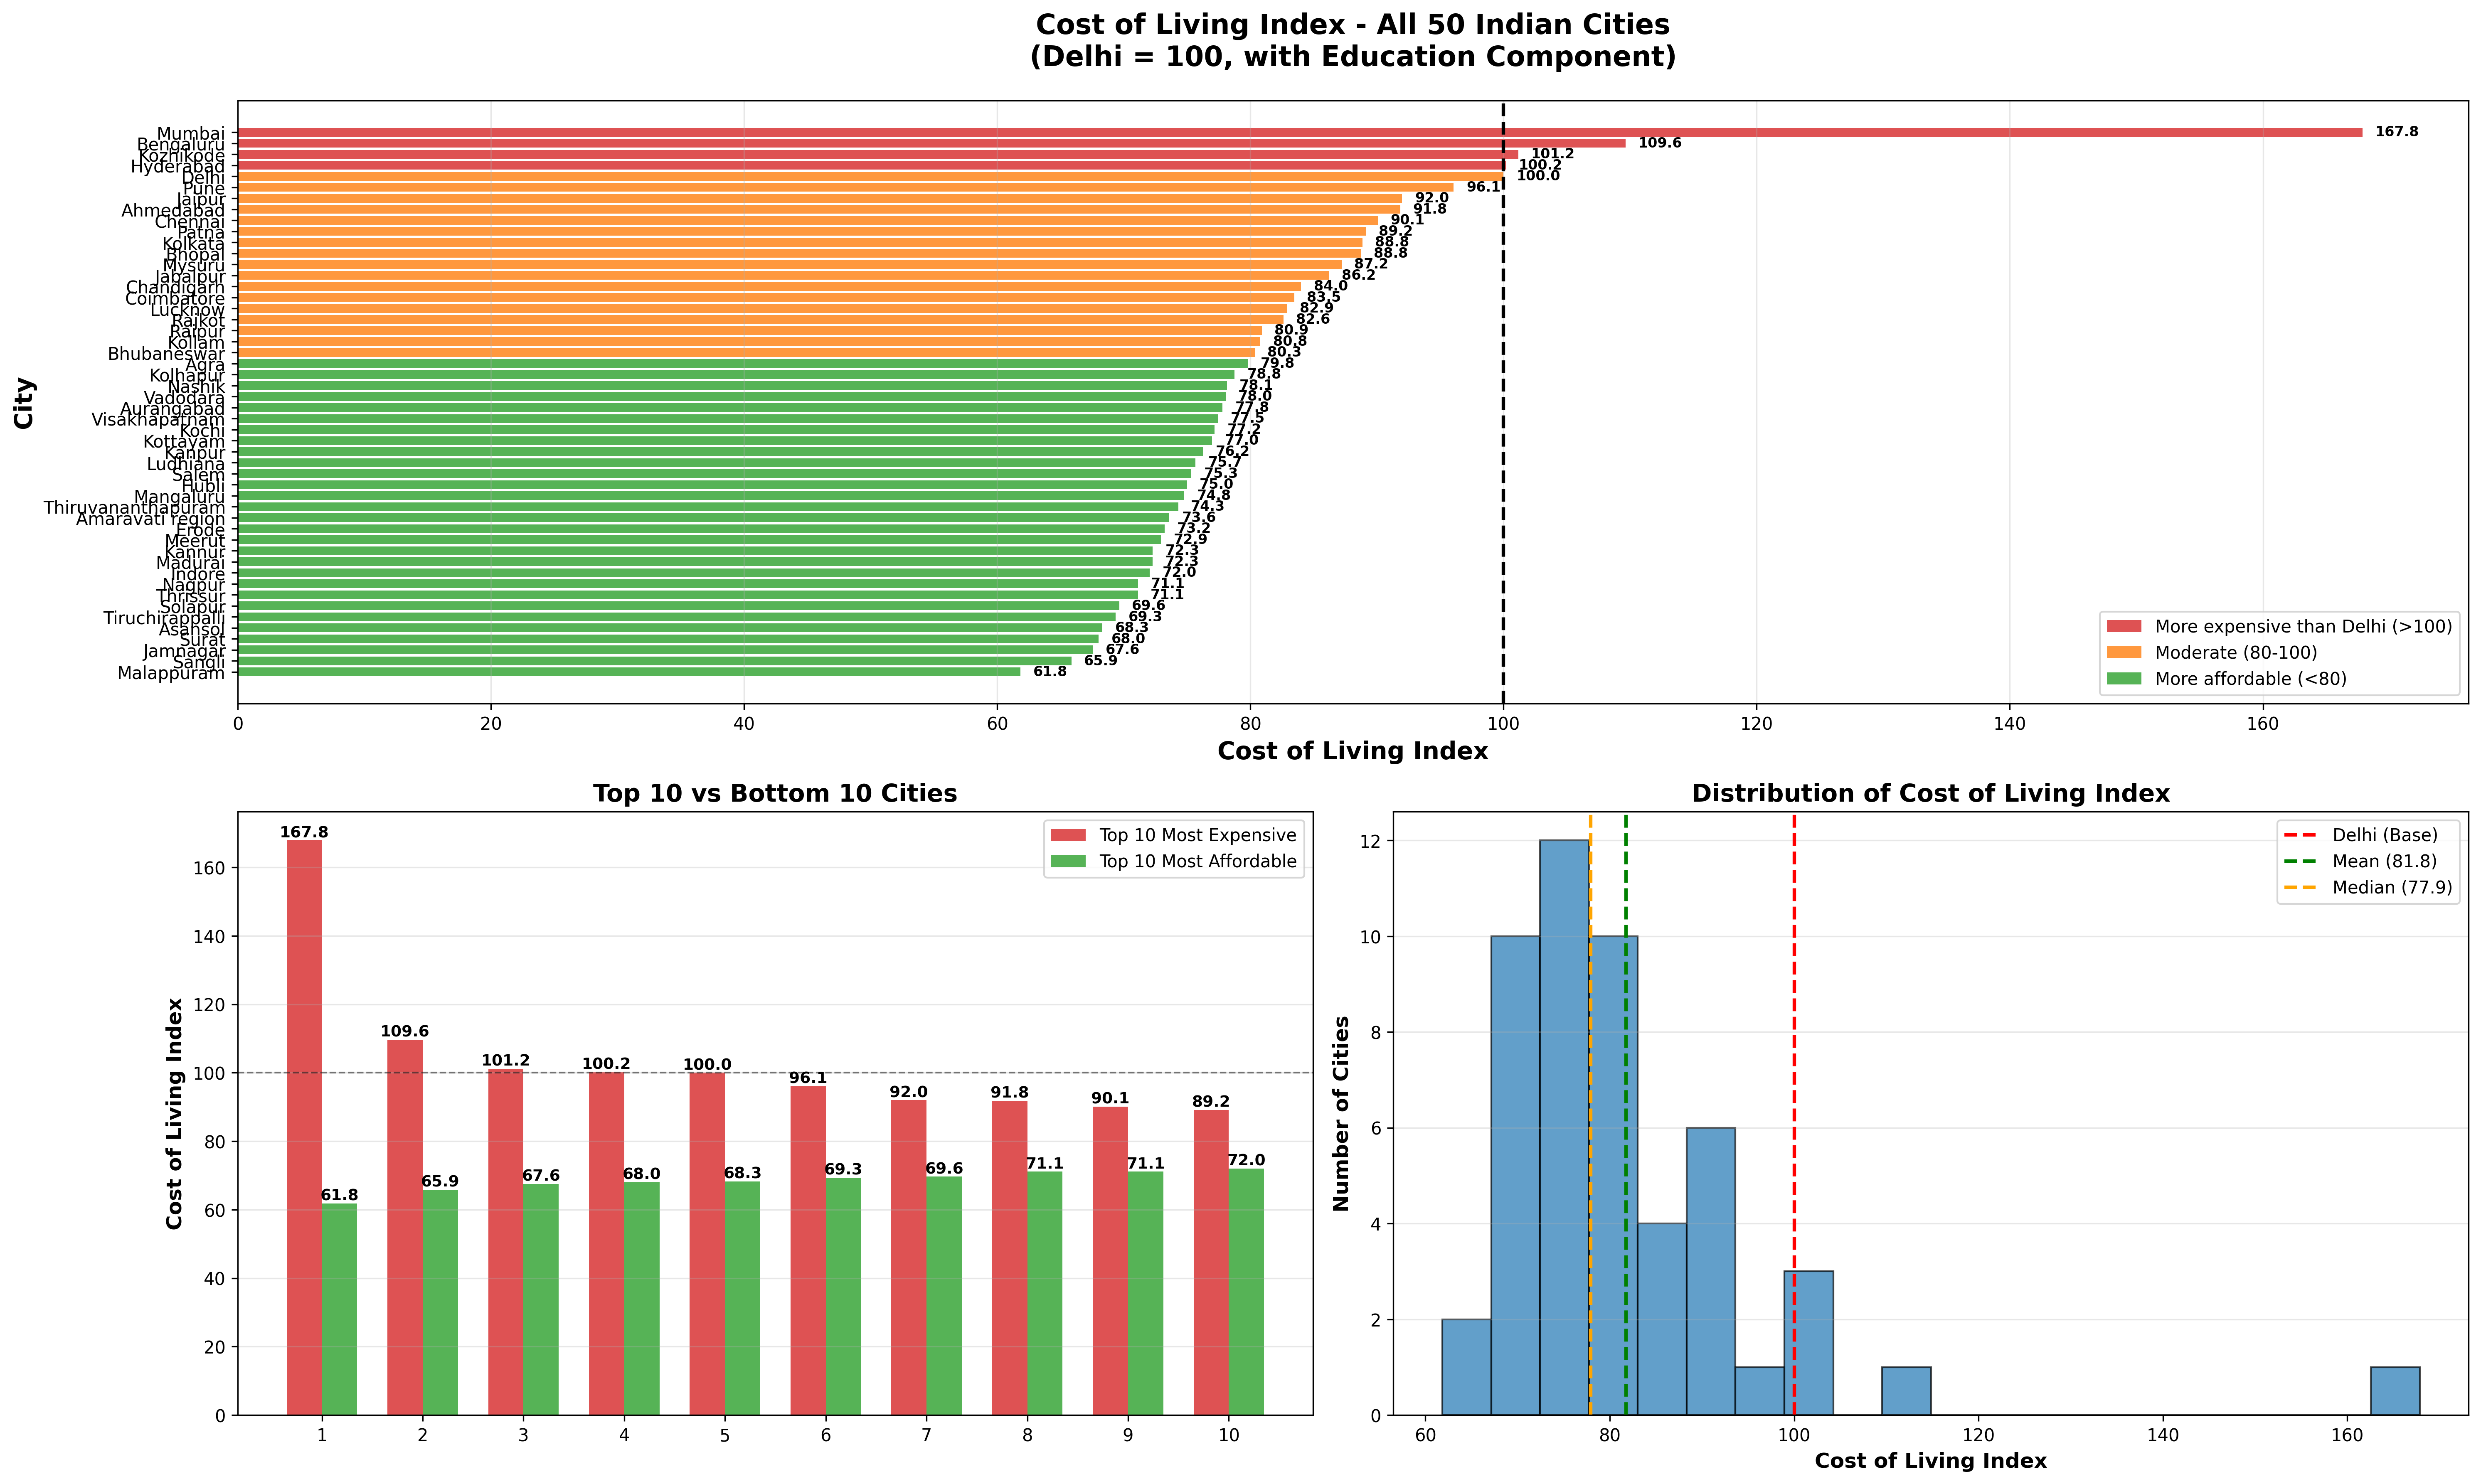
\includegraphics[width=\linewidth]{outputs/visualizations/cost_of_living_all_cities.png}
  \caption{Cost of Living Index -- all 50 cities (horizontal bar chart)}
\end{figure}

\begin{figure}[H]
  \centering
  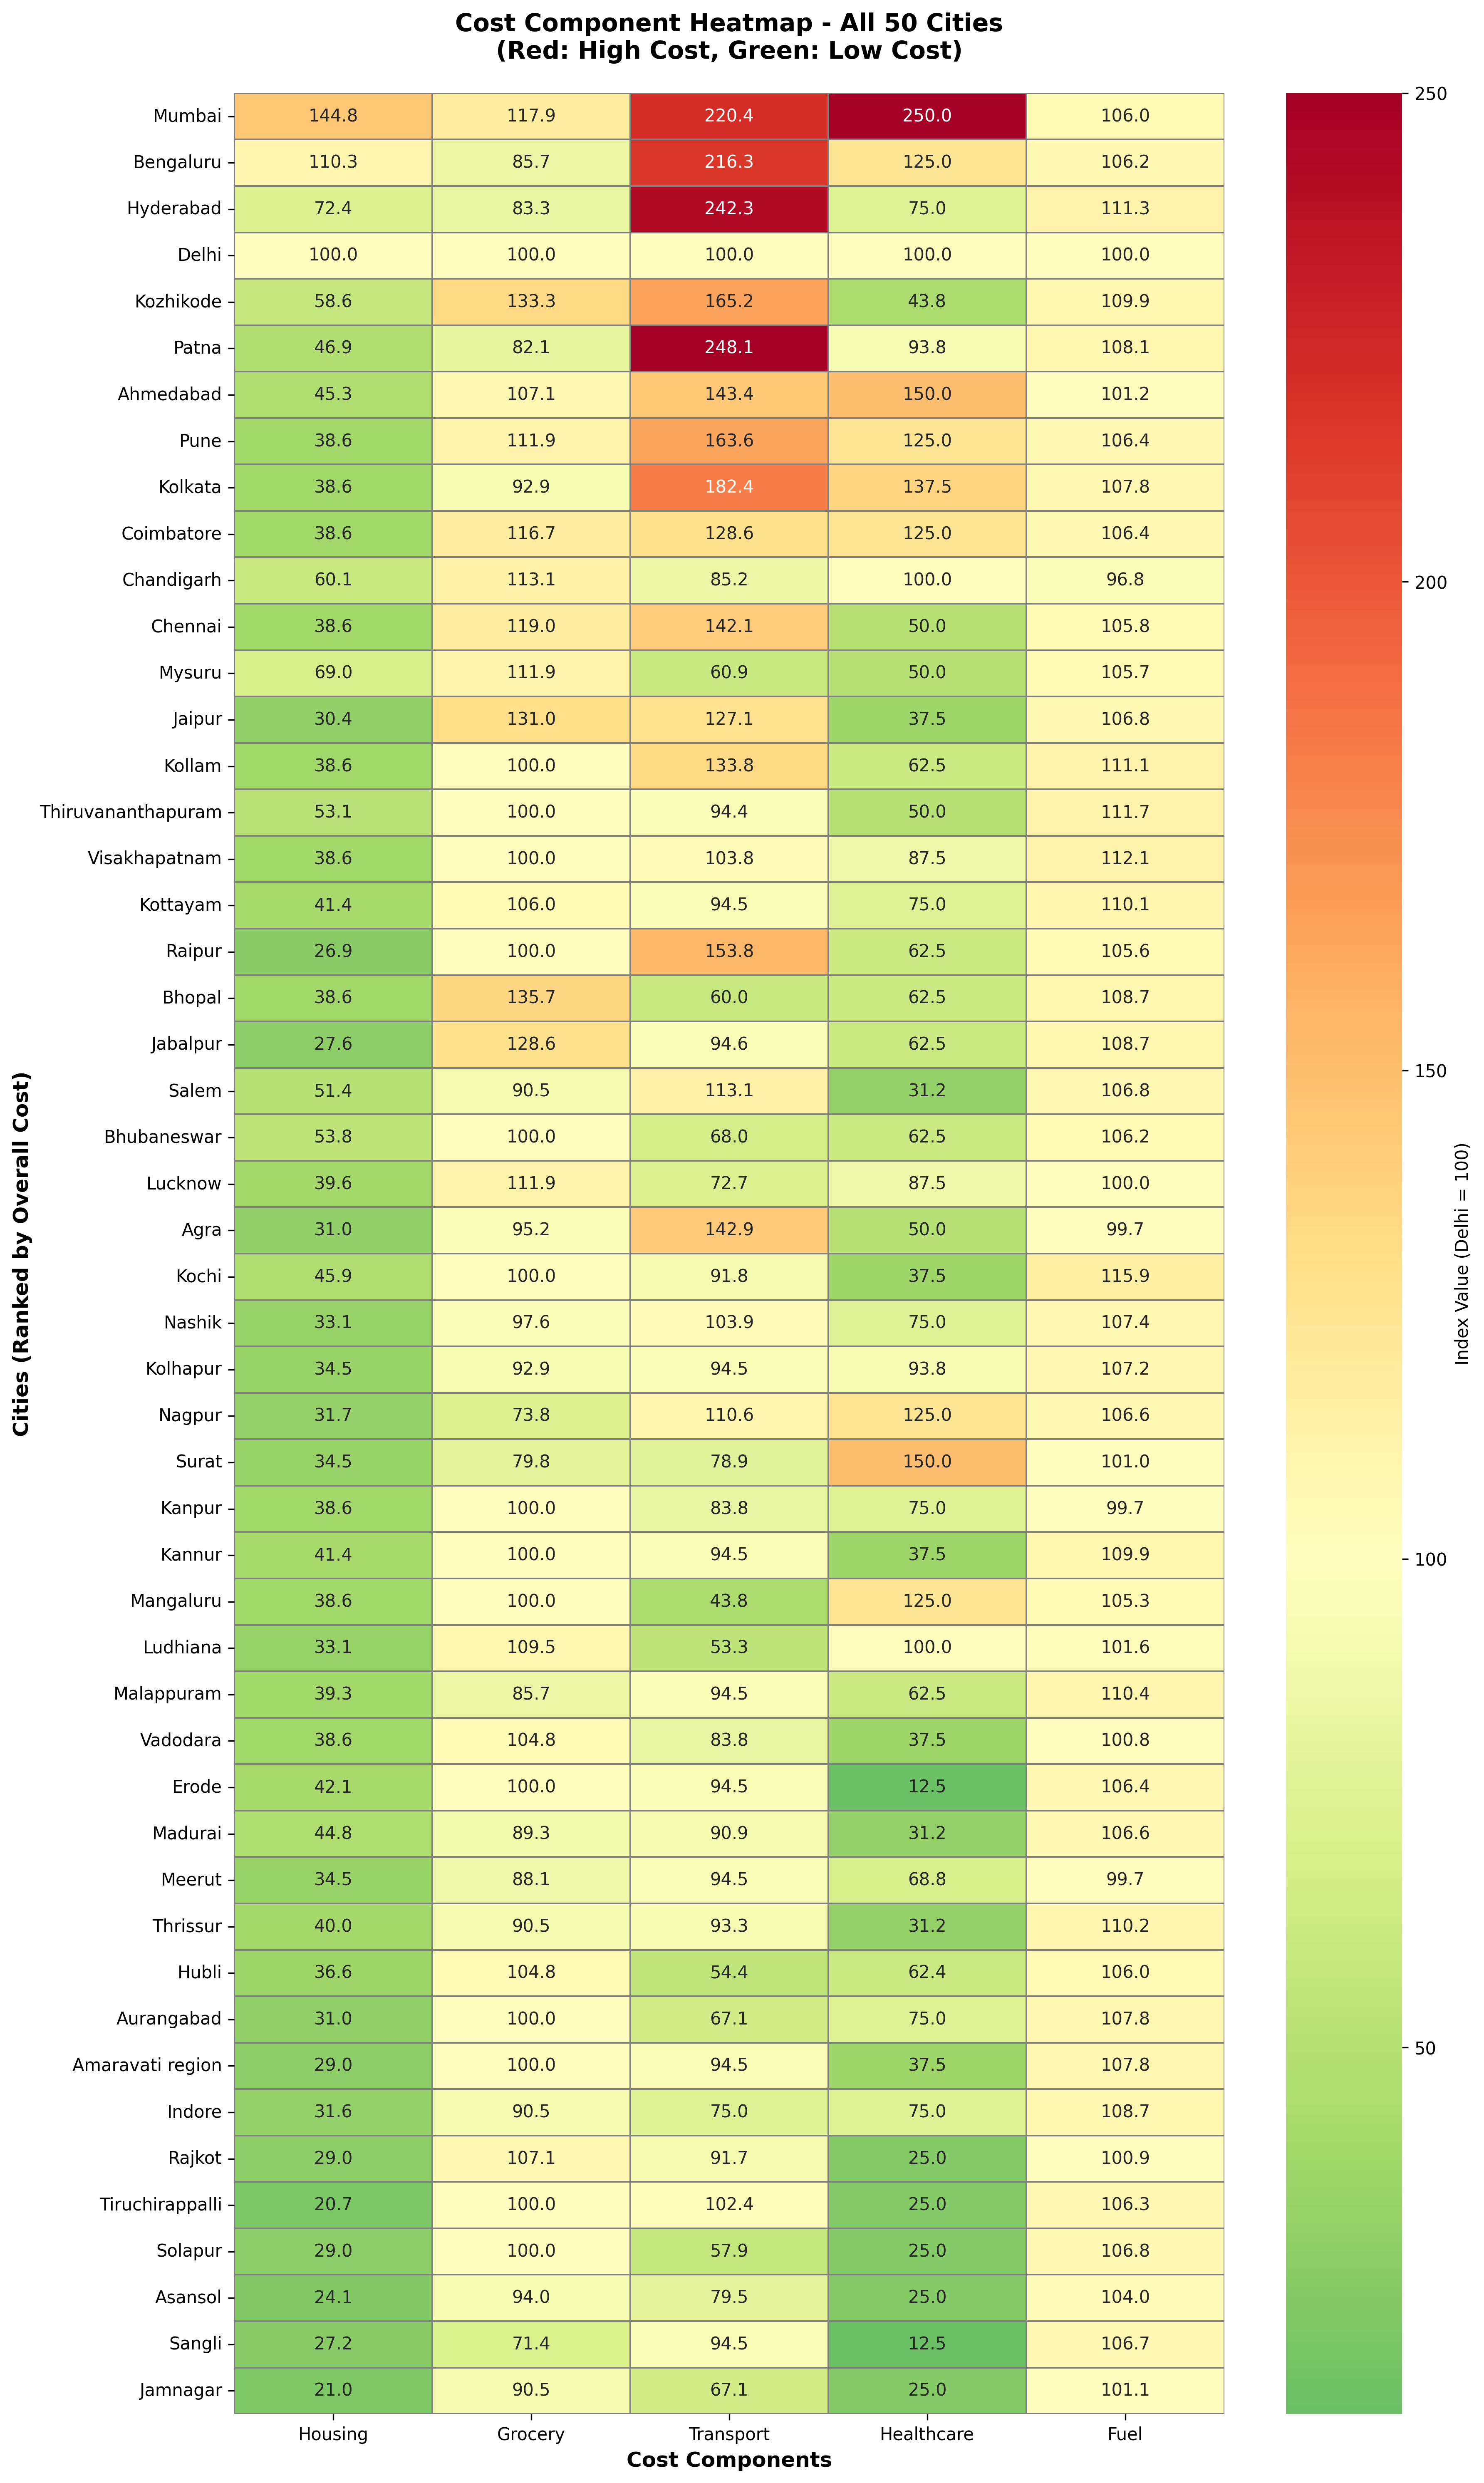
\includegraphics[width=\linewidth]{outputs/visualizations/heatmap_all_50_cities.png}
  \caption{Component heatmap -- all 50 cities across all 8 cost dimensions}
\end{figure}

\begin{figure}[H]
  \centering
  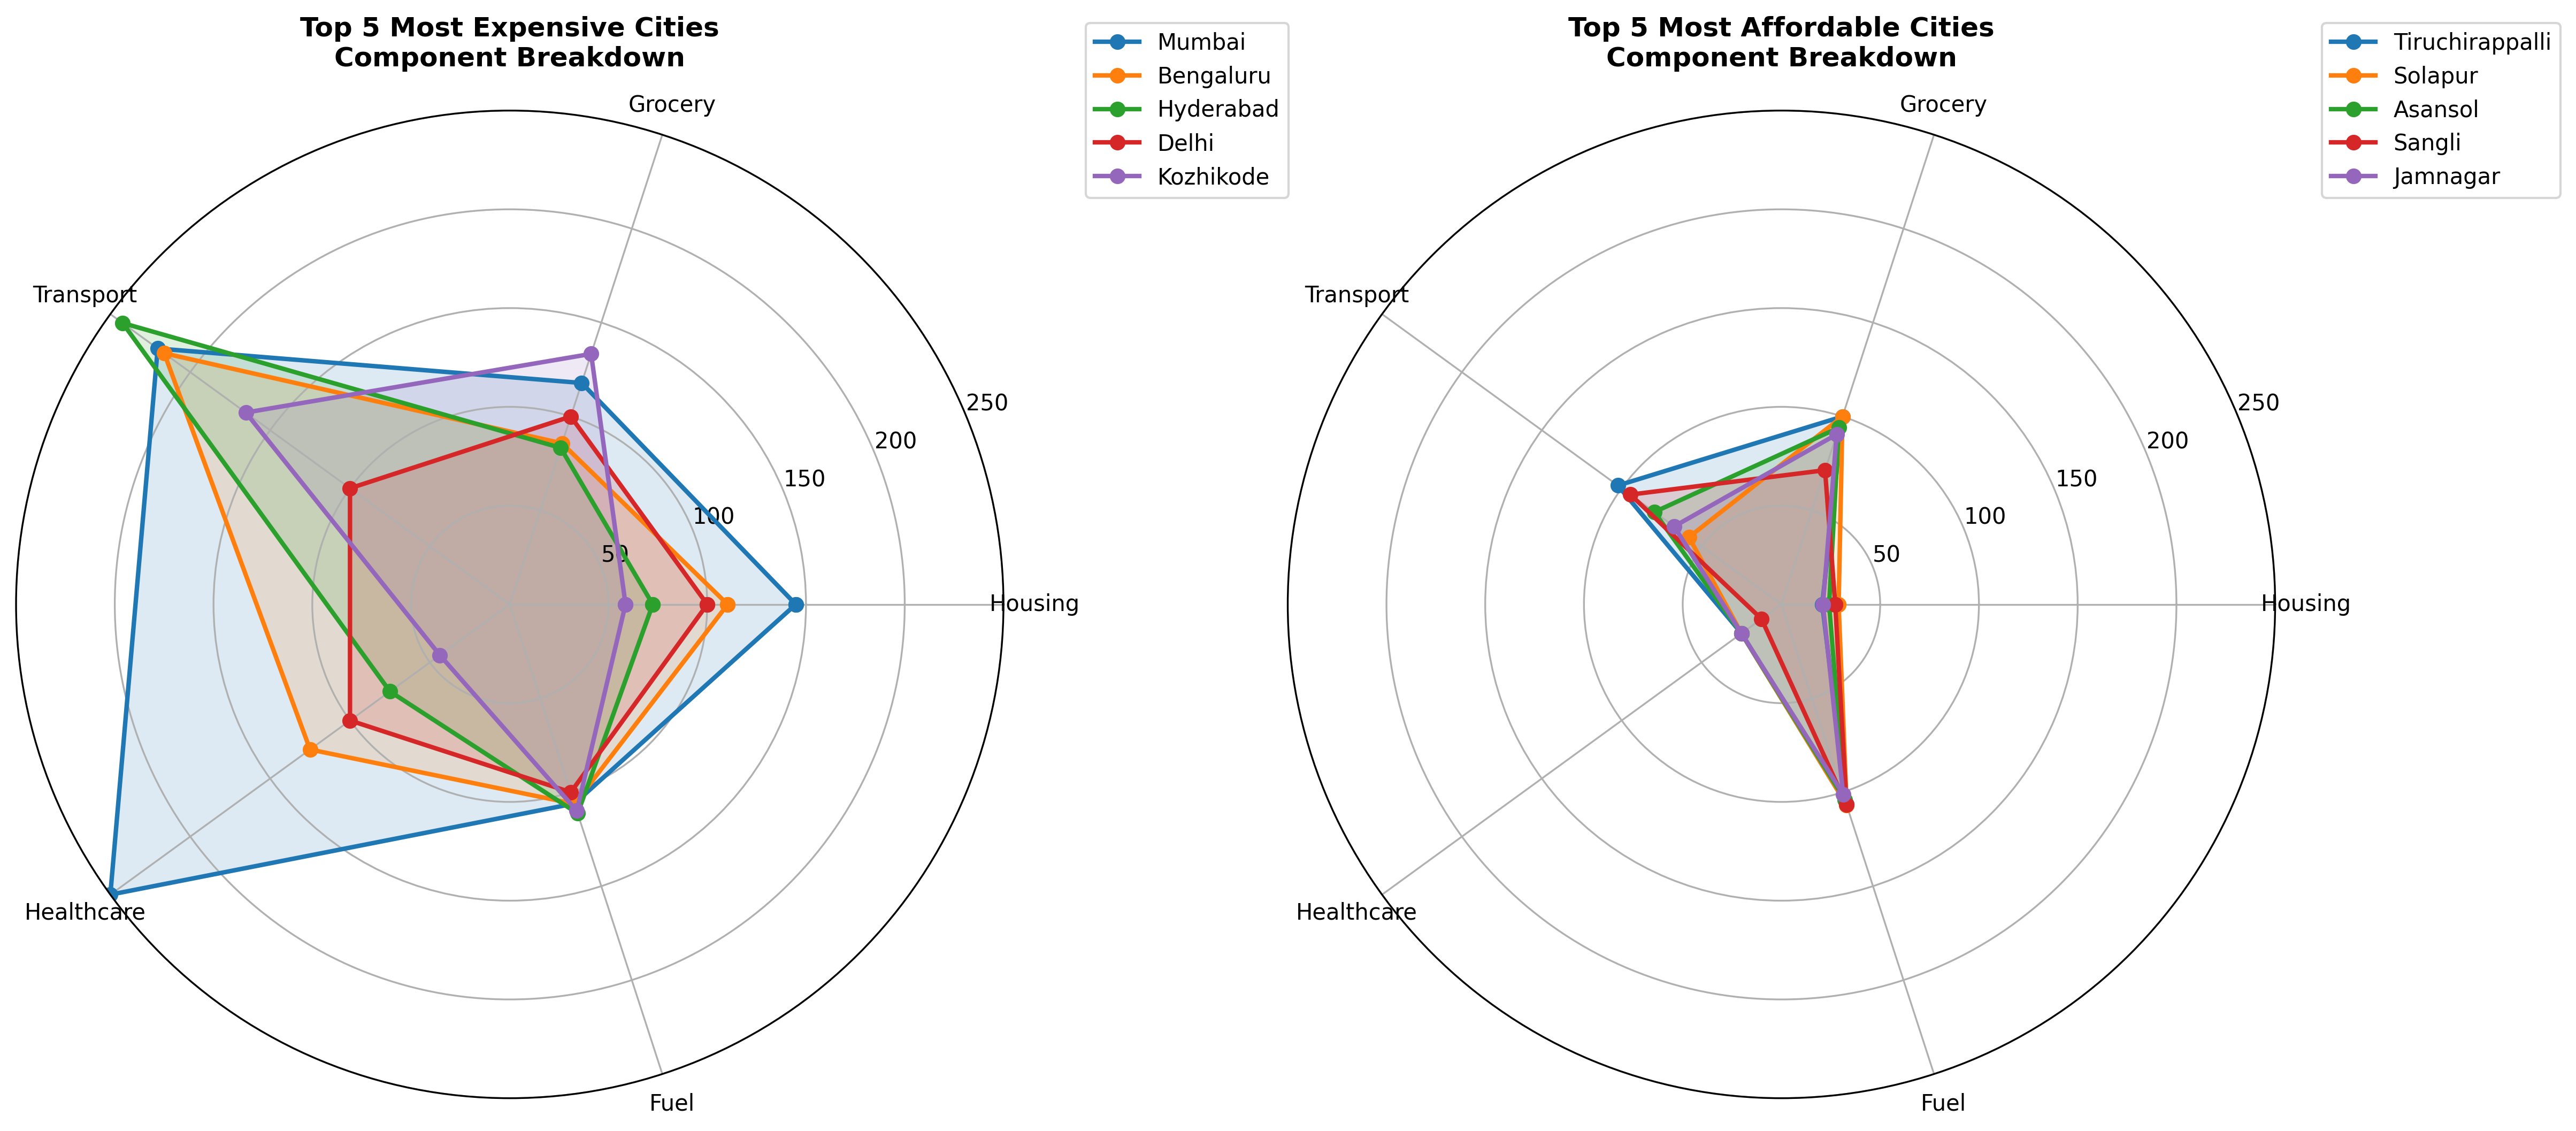
\includegraphics[width=\linewidth]{outputs/visualizations/radar_chart_comparison.png}
  \caption{Radar chart comparing selected cities across all cost components}
\end{figure}

\begin{figure}[H]
  \centering
  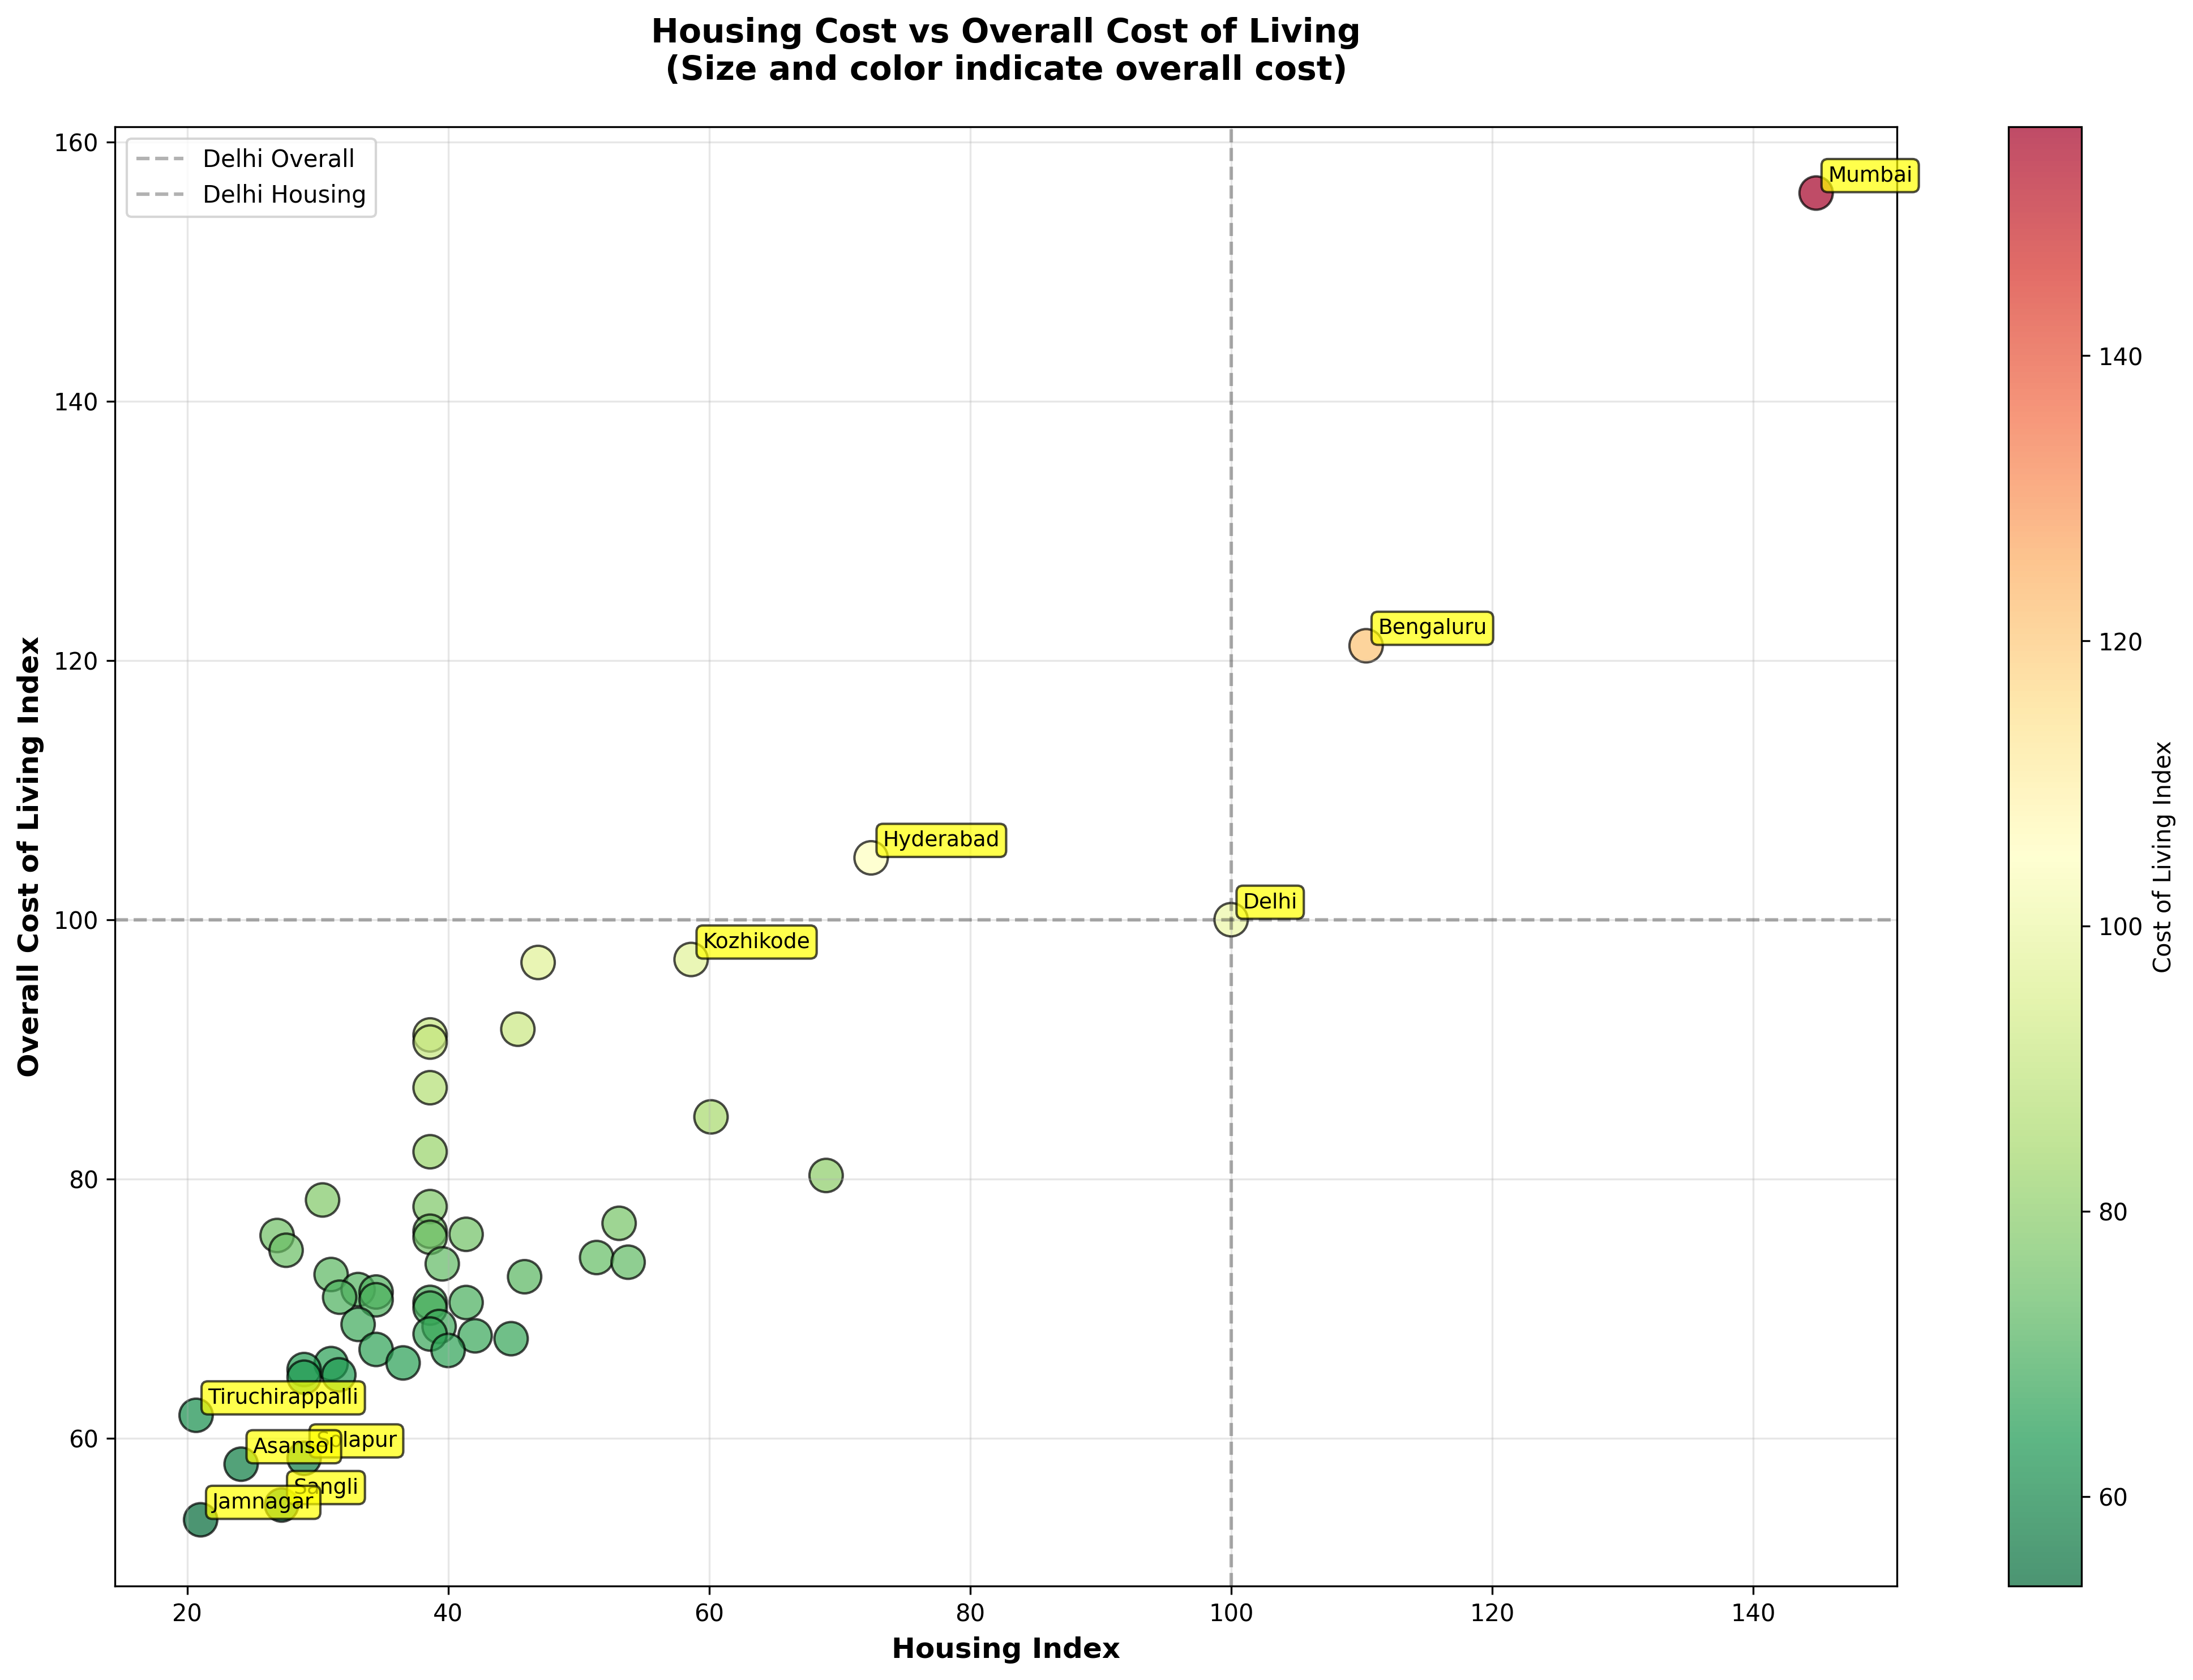
\includegraphics[width=0.85\linewidth]{outputs/visualizations/housing_vs_overall.png}
  \caption{Housing index vs. overall cost of living index (scatter plot)}
\end{figure}

\begin{figure}[H]
  \centering
  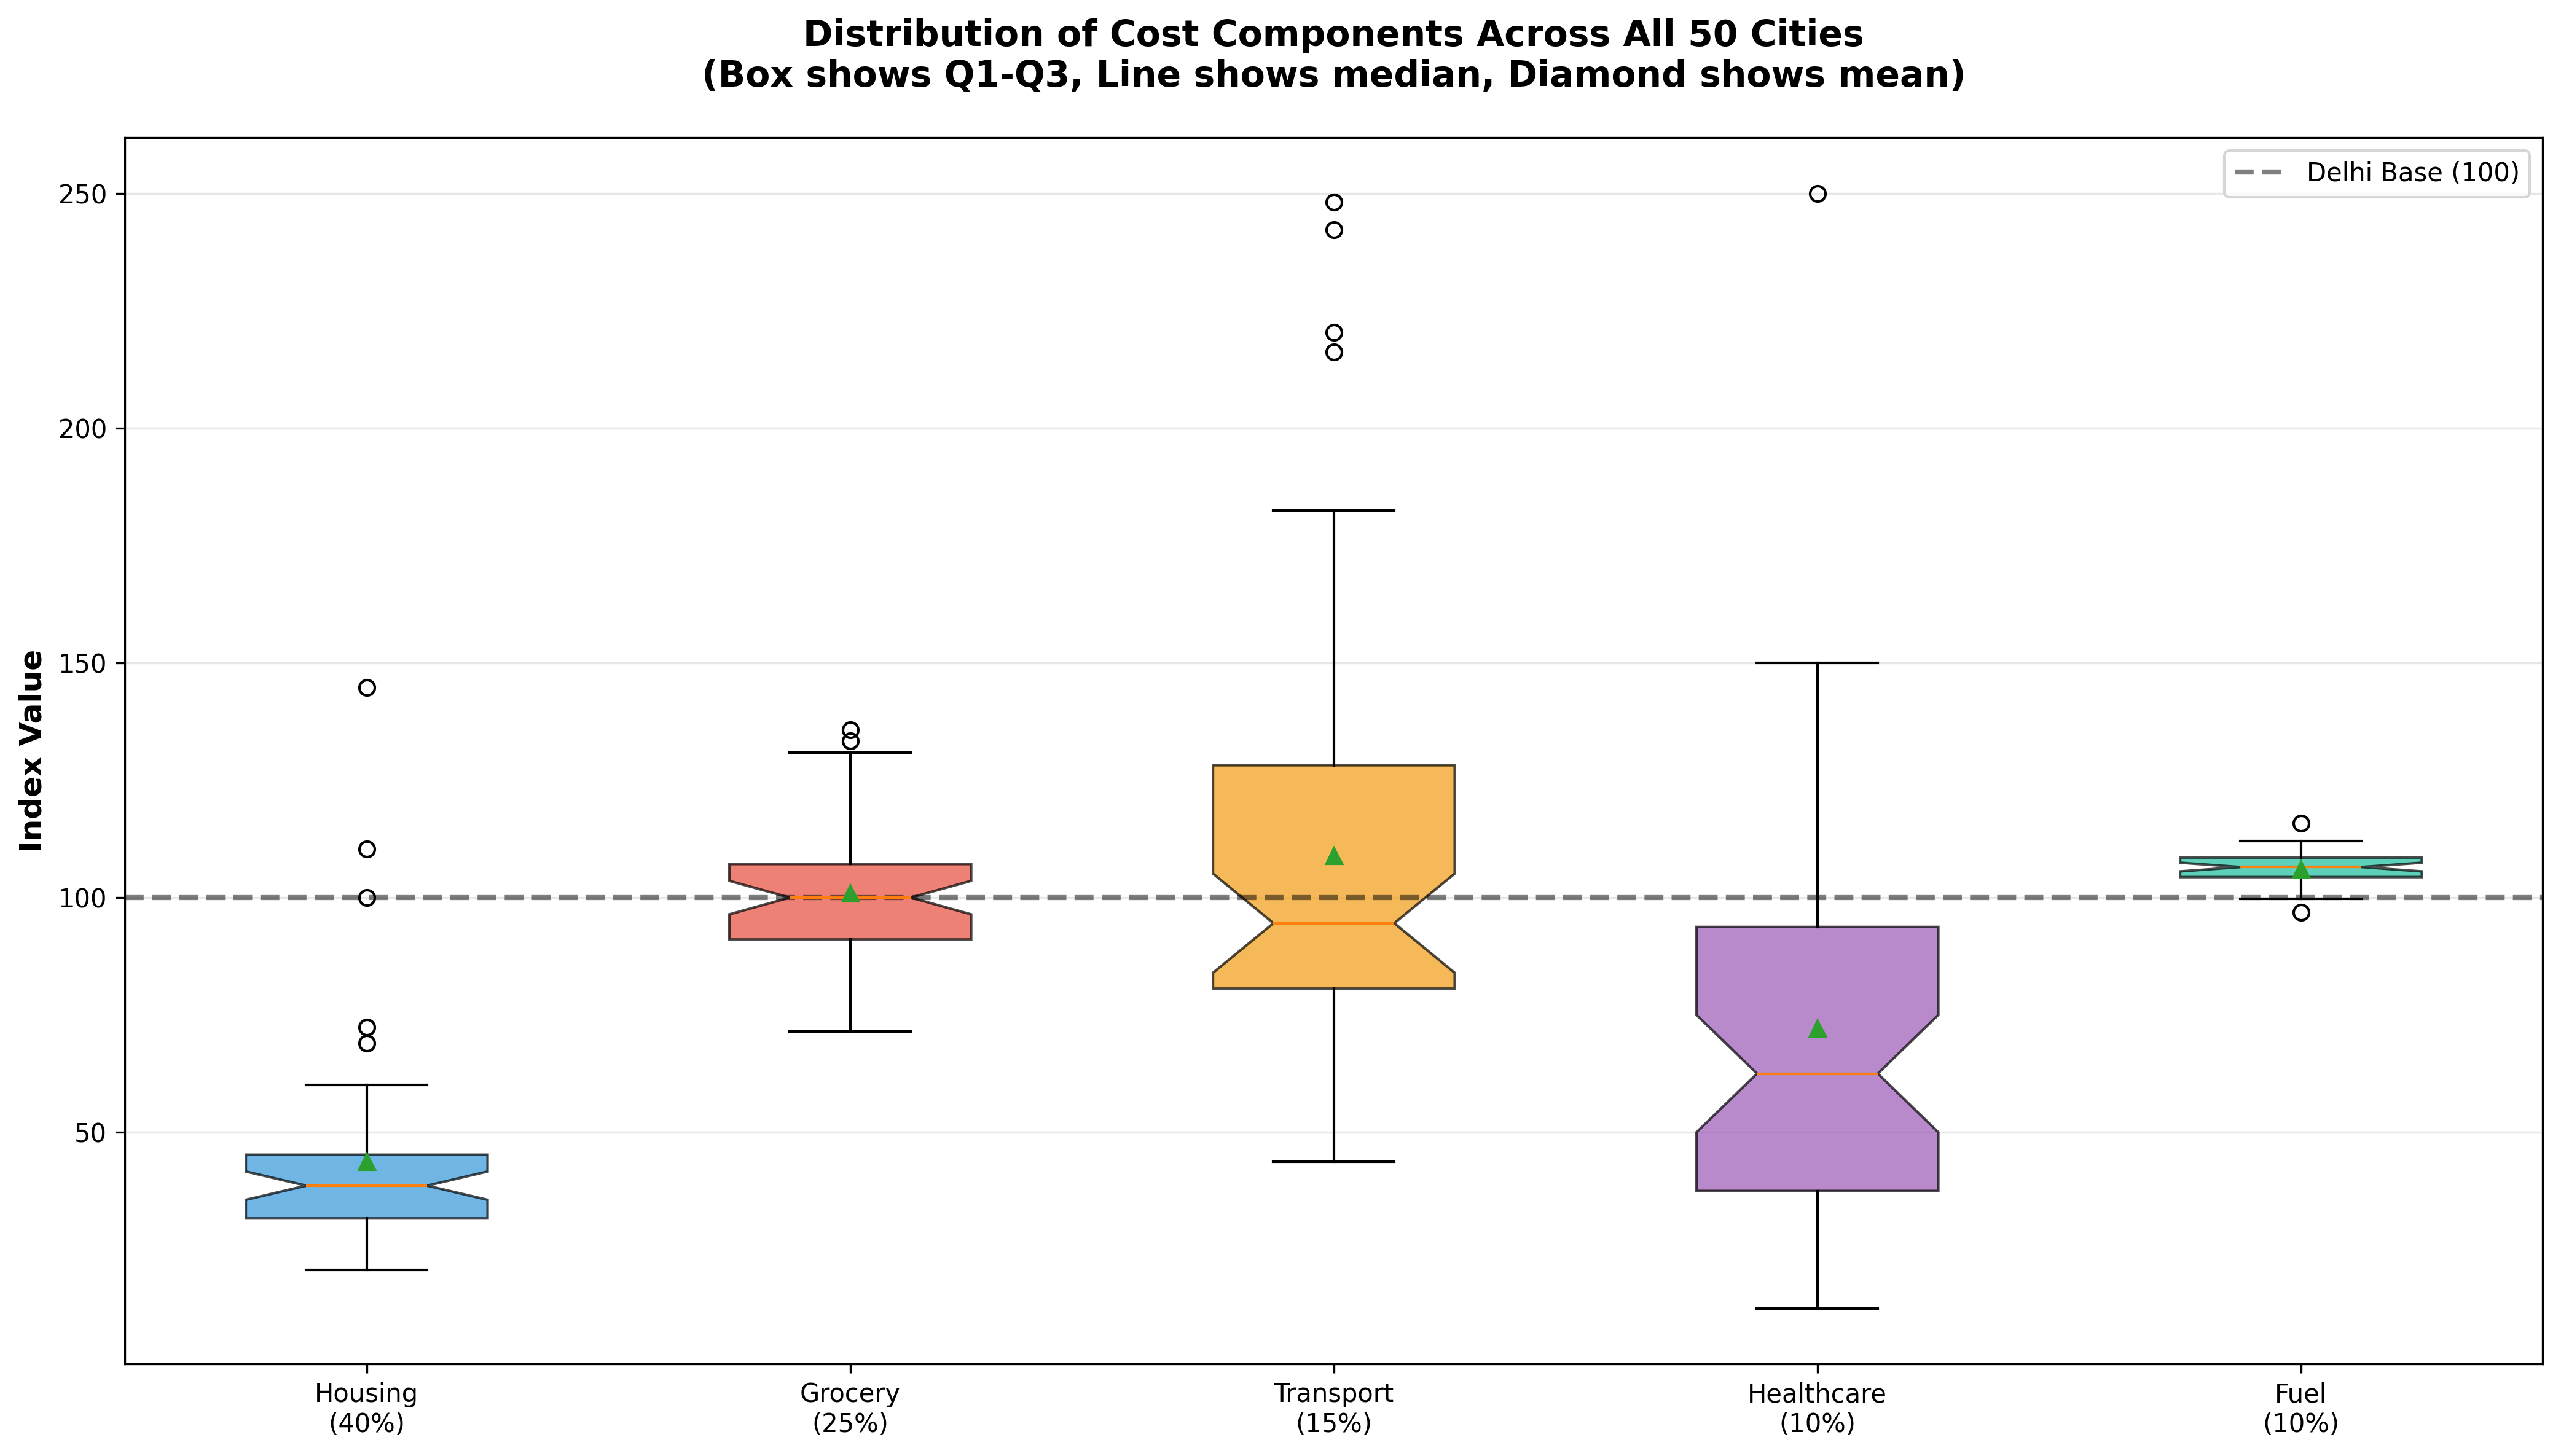
\includegraphics[width=0.8\linewidth]{outputs/visualizations/component_distribution_boxplot.png}
  \caption{Box plot distribution of each cost component across all 50 cities}
\end{figure}

\begin{figure}[H]
  \centering
  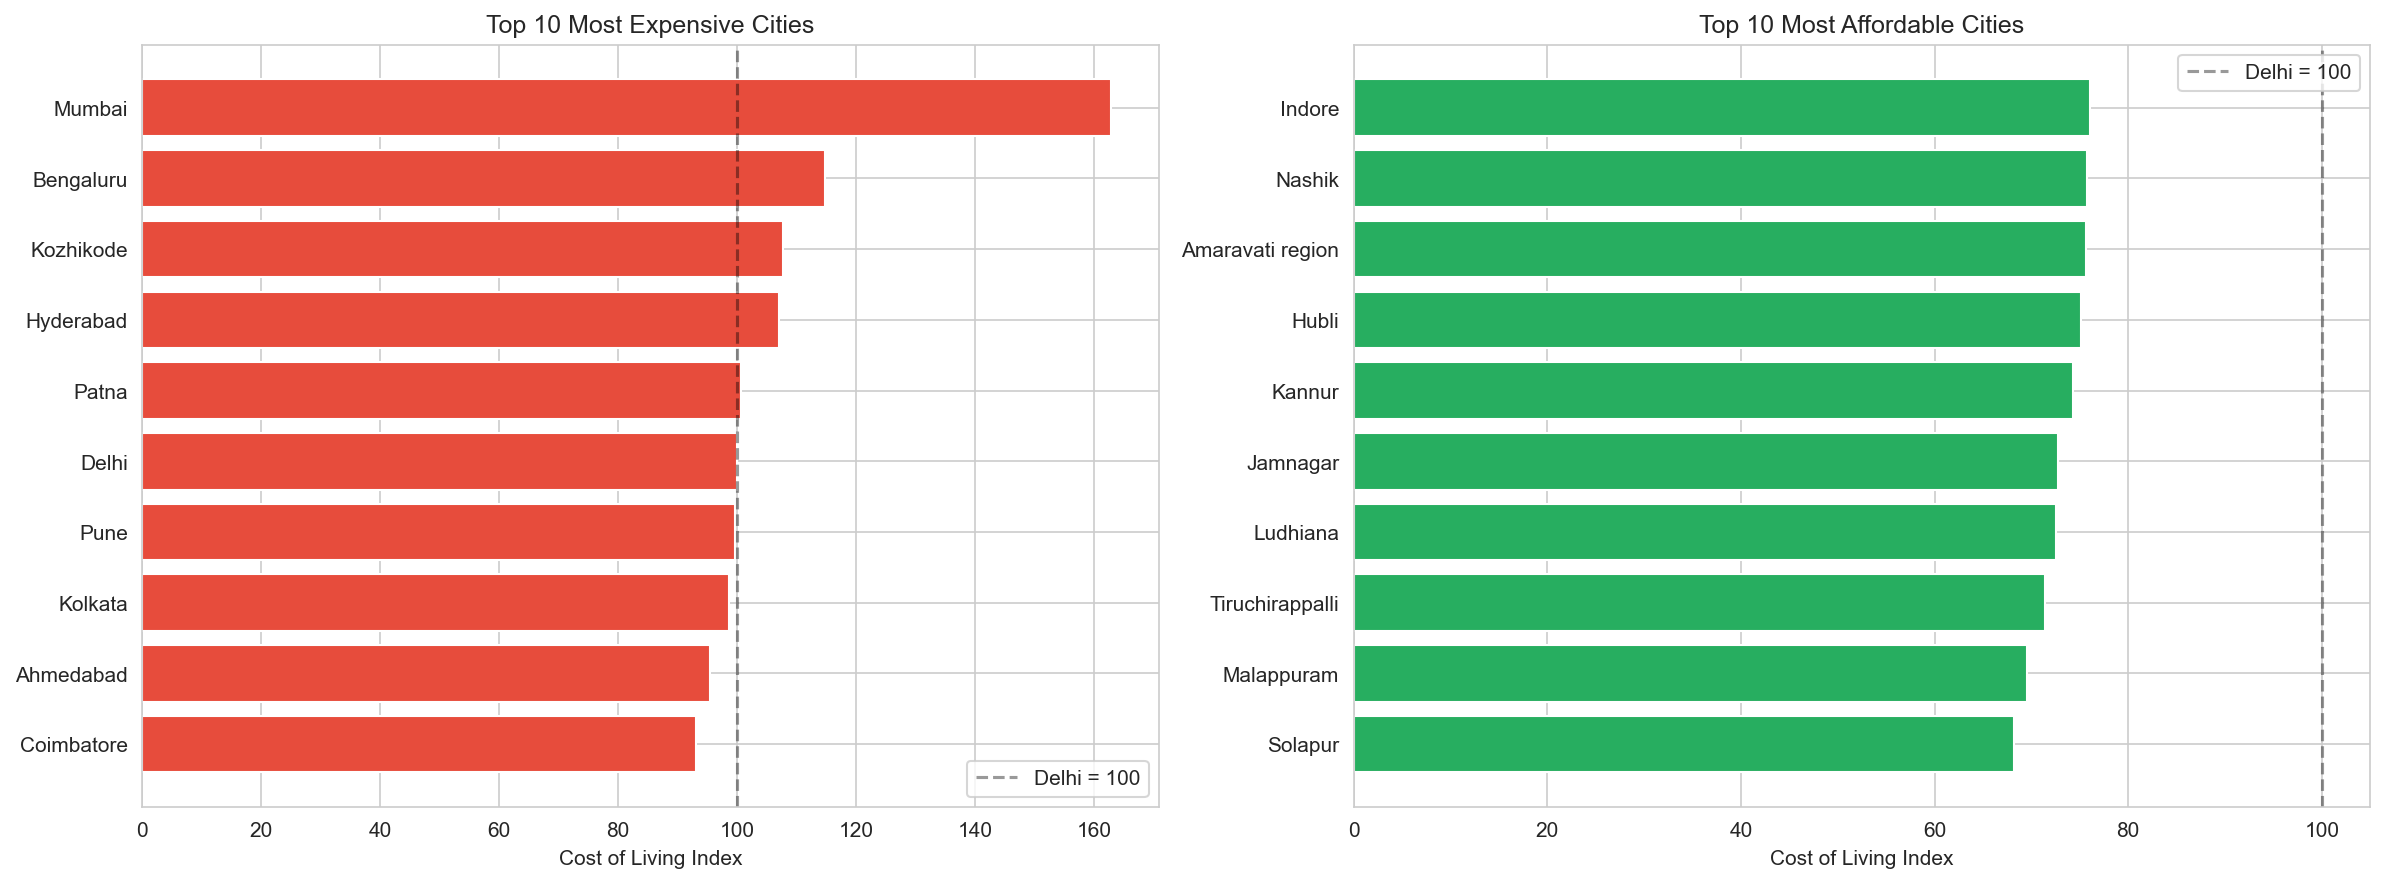
\includegraphics[width=0.75\linewidth]{outputs/visualizations/top_bottom_cities.png}
  \caption{Top 5 most expensive vs. top 5 most affordable cities}
\end{figure}

\begin{figure}[H]
  \centering
  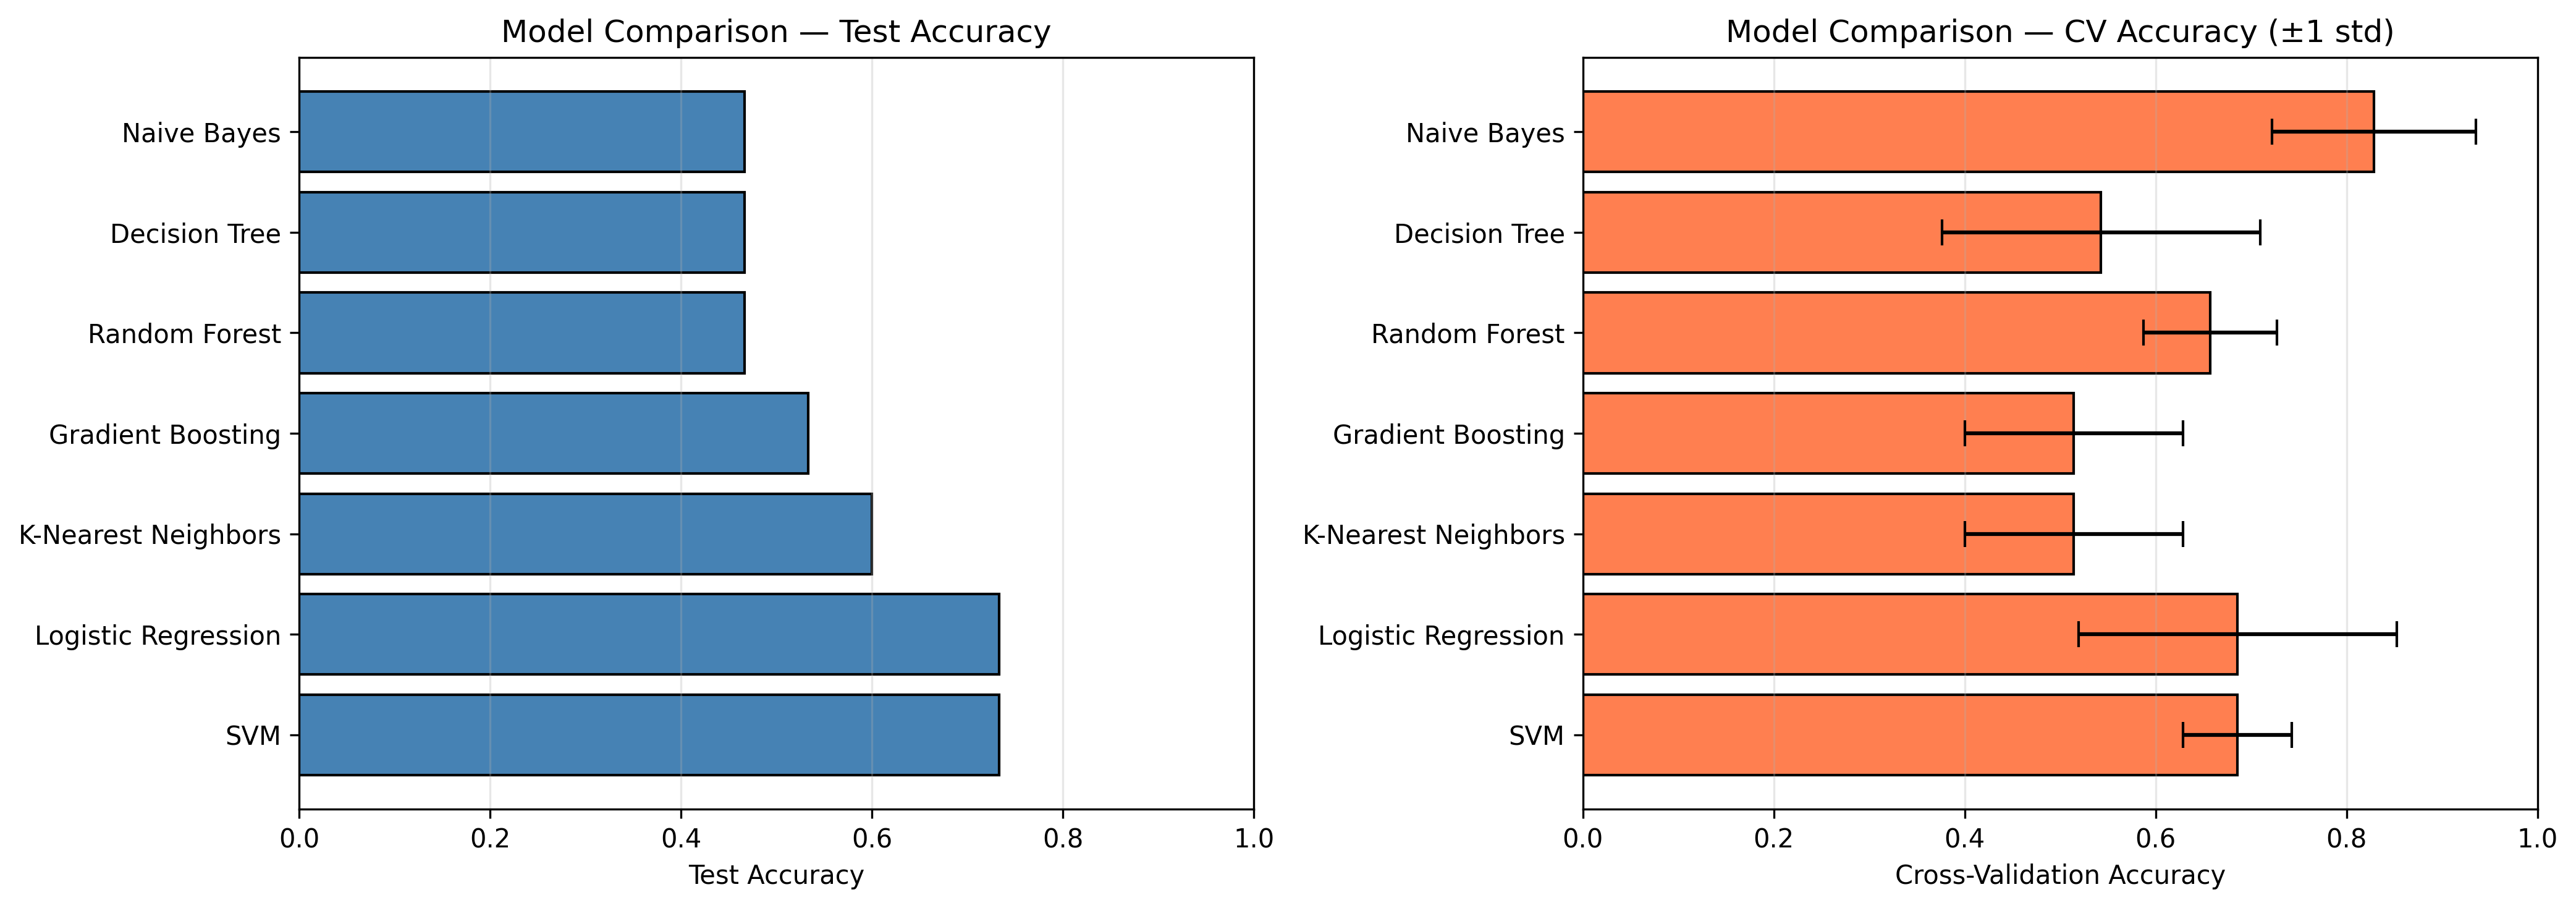
\includegraphics[width=0.75\linewidth]{outputs/visualizations/ml_algorithm_comparison.png}
  \caption{ML model accuracy comparison for city tier classification}
\end{figure}

\begin{figure}[H]
  \centering
  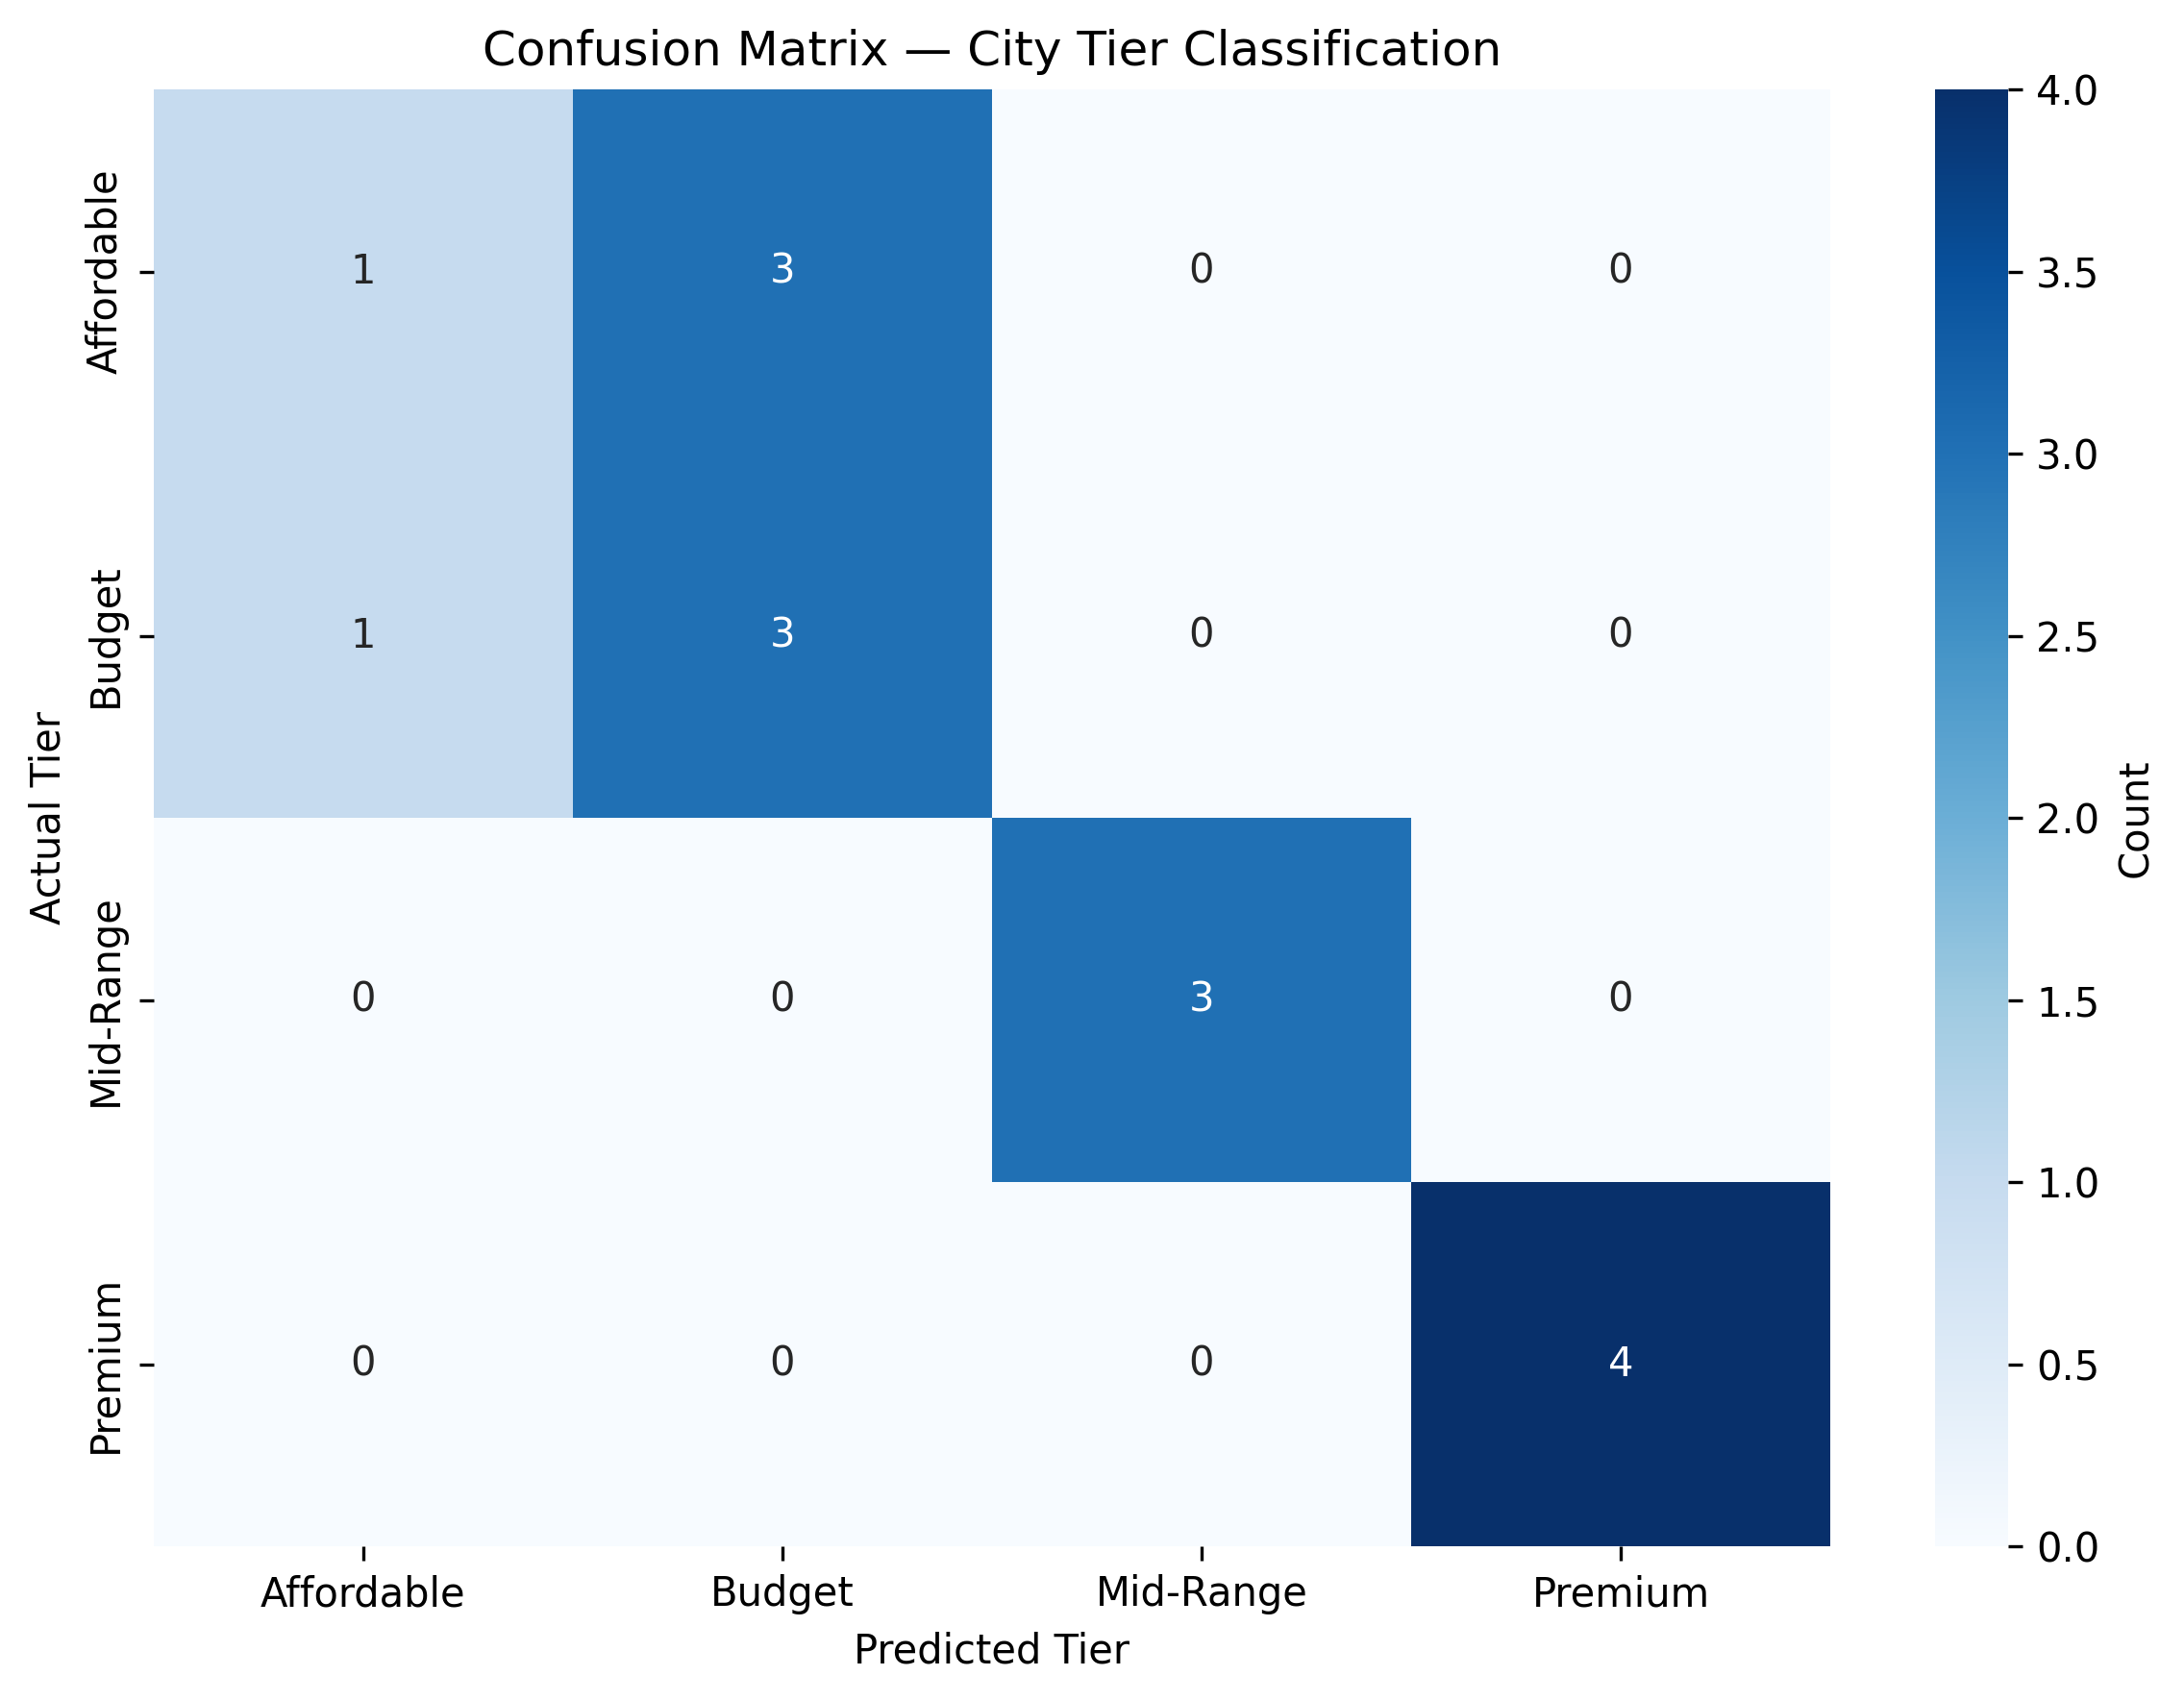
\includegraphics[width=0.7\linewidth]{outputs/visualizations/ml_confusion_matrix.png}
  \caption{Confusion matrix for the best-performing ML classifier}
\end{figure}

\begin{figure}[H]
  \centering
  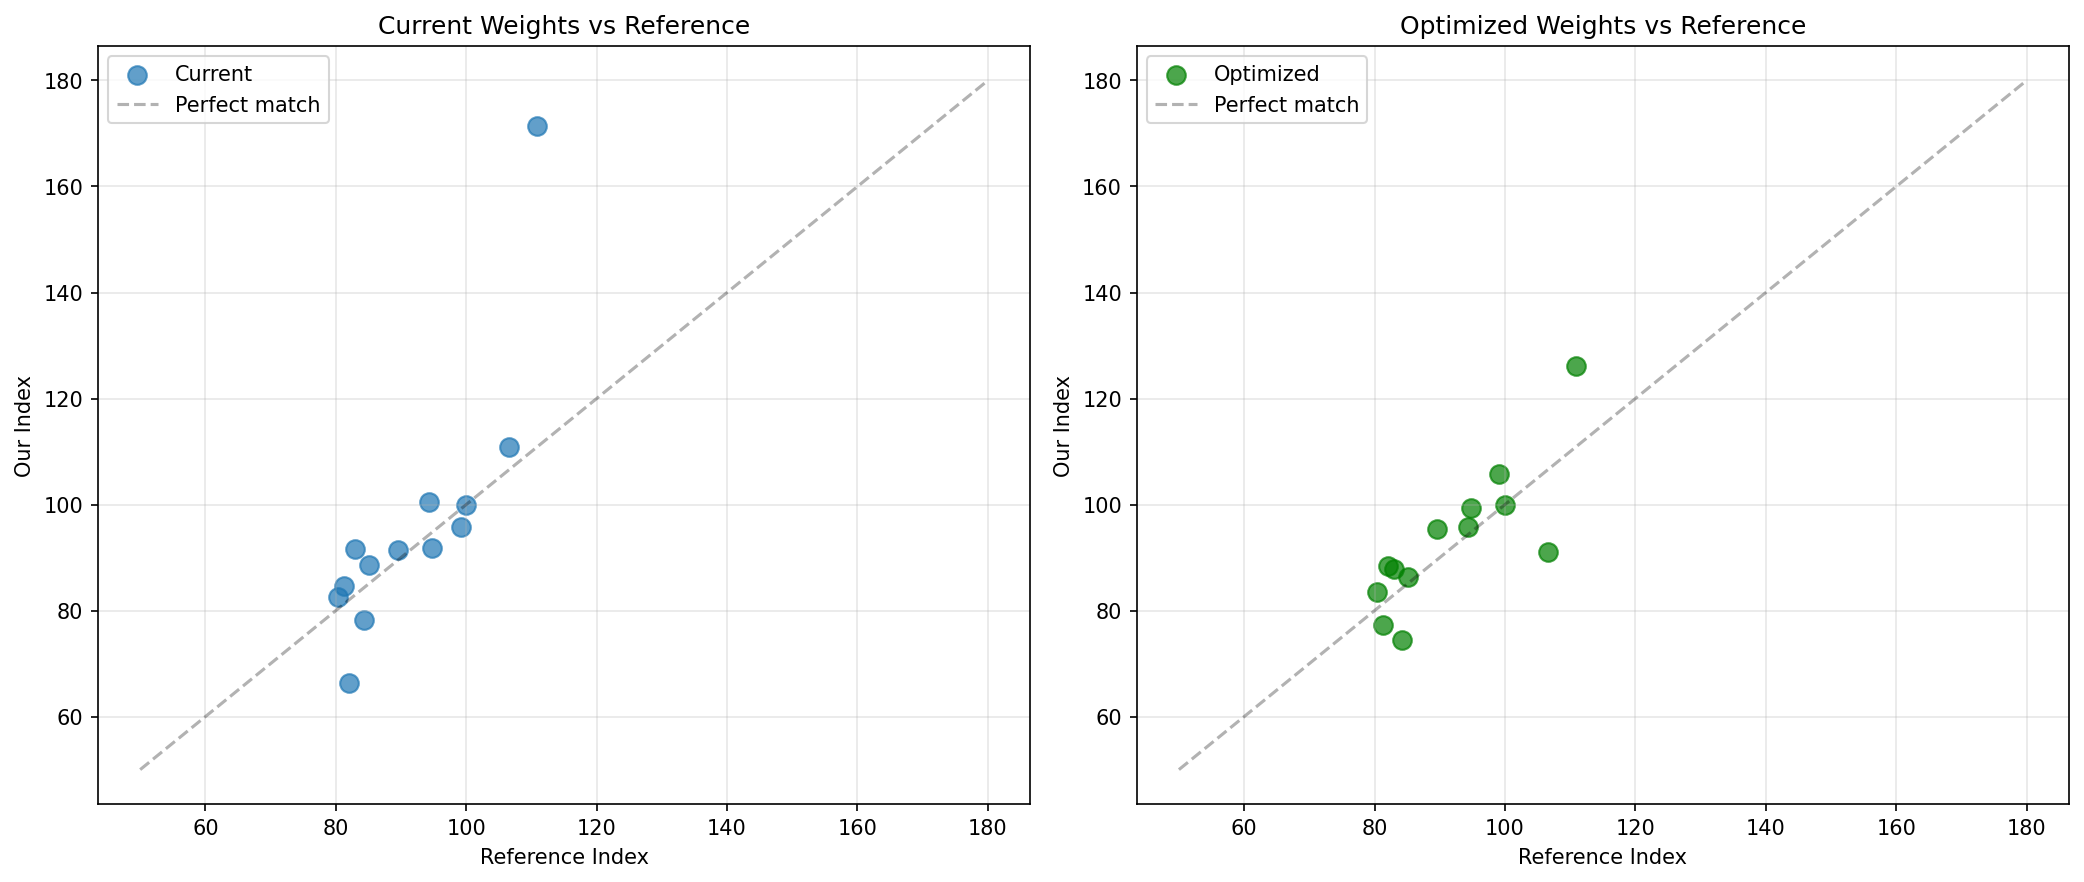
\includegraphics[width=0.75\linewidth]{outputs/visualizations/weight_optimization_comparison.png}
  \caption{City ranking comparison: original weights vs. optimised weights}
\end{figure}

\subsection{Full Visualization List}

\begin{longtable}{cll}
  \toprule
  \textbf{No.} & \textbf{File} & \textbf{Description} \\
  \midrule
  \endfirsthead
  \toprule
  \textbf{No.} & \textbf{File} & \textbf{Description} \\
  \midrule
  \endhead
  1  & \texttt{all\_50\_cities\_components.png}          & Component breakdown, all cities \\
  2  & \texttt{all\_50\_cities\_ranking.png}             & Overall ranking bar chart \\
  3  & \texttt{component\_breakdown.png}                 & Weighted contribution breakdown \\
  4  & \texttt{component\_distribution\_boxplot.png}     & Box plots per component \\
  5  & \texttt{components\_all\_cities.png}              & Multi-line component chart \\
  6  & \texttt{cost\_of\_living\_all\_cities.png}        & Horizontal bar, all cities \\
  7  & \texttt{cost\_of\_living\_components\_breakdown.png} & Stacked component chart \\
  8  & \texttt{dining\_entertainment.png}                & Restaurant \& movie index \\
  9  & \texttt{distribution.png}                         & Index distribution histogram \\
  10 & \texttt{education\_cost\_comparison.png}          & City-wise tutor fees \\
  11 & \texttt{electricity\_index.png}                   & Electricity rate index \\
  12 & \texttt{heatmap.png}                              & Component heatmap (sample) \\
  13 & \texttt{heatmap\_all\_50\_cities.png}             & Full 50-city heatmap \\
  14 & \texttt{housing\_vs\_overall.png}                 & Housing vs. overall index \\
  15 & \texttt{ml\_algorithm\_comparison.png}            & ML model comparison \\
  16 & \texttt{ml\_confusion\_matrix.png}                & ML confusion matrix \\
  17 & \texttt{movie\_ticket\_index.png}                 & Movie ticket index \\
  18 & \texttt{overall\_index\_all\_cities.png}          & Overall index bar chart \\
  19 & \texttt{radar\_chart\_comparison.png}             & Radar chart \\
  20 & \texttt{restaurant\_index.png}                    & Restaurant price index \\
  21 & \texttt{top\_bottom\_cities.png}                  & Top/bottom 5 comparison \\
  22 & \texttt{weight\_optimization\_comparison.png}     & Weight sensitivity analysis \\
  23 & \texttt{weighted\_contribution\_stacked.png}      & Stacked weighted contribution \\
  \bottomrule
\end{longtable}

% ─────────────────────────────────────────────────────────────────────────
\section{Key Findings}

\subsection{Full City Rankings}

\begin{longtable}{clcc}
  \toprule
  \textbf{Rank} & \textbf{City} & \textbf{Index} & \textbf{Category} \\
  \midrule
  \endfirsthead
  \toprule
  \textbf{Rank} & \textbf{City} & \textbf{Index} & \textbf{Category} \\
  \midrule
  \endhead
  1  & Mumbai             & 162.79 & Expensive \\
  2  & Bengaluru          & 114.76 & Expensive \\
  3  & Kozhikode          & 107.66 & Expensive \\
  4  & Hyderabad          & 107.09 & Expensive \\
  5  & Patna              & 100.72 & Expensive \\
  6  & Delhi              & 100.00 & Base City \\
  7  & Pune               &  99.61 & Moderate \\
  8  & Kolkata            &  98.57 & Moderate \\
  9  & Ahmedabad          &  95.42 & Moderate \\
  10 & Coimbatore         &  93.04 & Moderate \\
  11 & Chennai            &  92.25 & Moderate \\
  12 & Raipur             &  89.95 & Moderate \\
  13 & Bhubaneswar        &  89.18 & Moderate \\
  14 & Jaipur             &  88.38 & Moderate \\
  15 & Rajkot             &  85.78 & Moderate \\
  16 & Bhopal             &  85.25 & Moderate \\
  17 & Jabalpur           &  84.32 & Moderate \\
  18 & Sangli             &  83.17 & Moderate \\
  19 & Agra               &  82.75 & Moderate \\
  20 & Thrissur           &  82.52 & Moderate \\
  21 & Salem              &  81.95 & Affordable \\
  22 & Mysuru             &  81.08 & Affordable \\
  23 & Kollam             &  81.05 & Affordable \\
  24 & Nagpur             &  81.03 & Affordable \\
  25 & Kolhapur           &  80.48 & Affordable \\
  26 & Lucknow            &  80.41 & Affordable \\
  27 & Erode              &  80.35 & Affordable \\
  28 & Chandigarh         &  80.16 & Affordable \\
  29 & Aurangabad         &  79.87 & Affordable \\
  30 & Visakhapatnam      &  79.52 & Affordable \\
  31 & Kochi              &  79.24 & Affordable \\
  32 & Kanpur             &  79.21 & Affordable \\
  33 & Asansol            &  78.39 & Affordable \\
  34 & Vadodara           &  77.82 & Affordable \\
  35 & Madurai            &  77.63 & Affordable \\
  36 & Meerut             &  77.60 & Affordable \\
  37 & Kottayam           &  77.11 & Affordable \\
  38 & Mangaluru          &  76.59 & Affordable \\
  39 & Surat              &  76.49 & Affordable \\
  40 & Thiruvananthapuram &  76.36 & Affordable \\
  41 & Indore             &  76.10 & Affordable \\
  42 & Nashik             &  75.71 & Affordable \\
  43 & Amaravati          &  75.65 & Affordable \\
  44 & Hubli              &  75.10 & Affordable \\
  45 & Kannur             &  74.34 & Affordable \\
  46 & Jamnagar           &  72.77 & Affordable \\
  47 & Ludhiana           &  72.50 & Affordable \\
  48 & Tiruchirappalli    &  71.41 & Affordable \\
  49 & Solapur            &  68.20 & Very Affordable \\
  50 & Malappuram         &  69.54 & Very Affordable \\
  \bottomrule
  \caption{Complete city cost of living rankings}
\end{longtable}

\subsection{Component-Level Insights}

\begin{table}[H]
  \centering
  \begin{tabular}{lccp{4.5cm}}
    \toprule
    \textbf{Component} & \textbf{Highest City} & \textbf{Lowest City} & \textbf{Insight} \\
    \midrule
    Housing     & Mumbai (230.86)    & Malappuram (14.77) & 15x variation -- largest spread \\
    Grocery     & Kozhikode (151.21) & Nashik (90.94)     & About 65\% variation \\
    Transport   & Hyderabad (242.31) & Mangaluru (43.75)  & Uber pricing varies widely \\
    Healthcare  & Mumbai (135.0)     & Salem (15.0)       & 9x variation \\
    Education   & Rajkot (105.16)    & Salem (15.4)       & Online platform skew \\
    Electricity & Mumbai (212.5)     & Visakhapatnam (75) & State tariff differences \\
    Restaurant  & Mumbai (120)       & Kolkata (80)       & Moderate variation \\
    Movies      & Kozhikode (154)    & Salem (15.4)       & Theater concentration \\
    \bottomrule
  \end{tabular}
  \caption{Component-level extreme values and key insights}
\end{table}

% ─────────────────────────────────────────────────────────────────────────
\section{Machine Learning Applications}

\subsection{City Tier Classification}

Implemented in \texttt{src/ml\_classification.py}. Cities are labelled as
\textit{Expensive}, \textit{Moderate}, or \textit{Affordable} and multiple
classifiers are compared:

\begin{itemize}
  \item Random Forest
  \item Support Vector Machine (SVM)
  \item Decision Tree
  \item Logistic Regression
\end{itemize}

\subsection{City Recommendation System}

Interactive Streamlit web app (\texttt{website/app.py}) lets users set priorities
(``cheap housing'', ``don't care about movies'', etc.) and returns ranked city
recommendations using a priority-weighted cosine similarity approach.

\subsection{Weight Optimisation}

\texttt{src/weight\_optimizer.py} uses Scipy optimisation to find component weights
that minimise a cost function, providing a data-driven alternative to the manually
set expenditure-based weights.

\subsection{Potential Future ML Work}

\begin{enumerate}
  \item \textbf{Predictive modelling} -- Random Forest / XGBoost to estimate costs for new cities
  \item \textbf{Clustering} -- K-Means city grouping by cost profile
  \item \textbf{Anomaly detection} -- Isolation Forest to flag unusual pricing patterns
  \item \textbf{Time series forecasting} -- ARIMA / Prophet for cost trend tracking
  \item \textbf{NLP} -- Sentiment analysis on city living reviews
\end{enumerate}

% ─────────────────────────────────────────────────────────────────────────
\section{Project Architecture}

\begin{lstlisting}
BMP Data Modelling/
  data/
    raw/
      Magic Bricks data/       <- 50 housing CSV files
      grocery/blinkit_citywise/  <- 41 grocery Excel files
      transport/               <- Uber + fuel prices
      healthcare/              <- Doctor consultation fees
      education/               <- 60K+ tutor listings
      utilities/               <- Electricity tariffs
      entertainment/           <- Movies + restaurants
  src/
    main.py                    <- Pipeline orchestrator
    data_loader.py             <- Load & preprocess all sources
    cost_calculator.py         <- Index formula & weighting
    visualizer.py              <- 23 chart types
    ml_classification.py       <- City tier ML models
    weight_optimizer.py        <- Optimal weight search
    recommender.py             <- City recommendation logic
  website/
    app.py                     <- Streamlit web interface
  outputs/
    reports/cost_index_results.csv   <- Full results (50 cities)
    visualizations/                  <- 23 PNG charts
\end{lstlisting}

\textbf{Technology Stack:}

\begin{itemize}
  \item Language: Python 3.8+
  \item Data processing: \texttt{pandas}, \texttt{numpy}
  \item Visualisation: \texttt{matplotlib}, \texttt{seaborn}
  \item Web interface: \texttt{streamlit}
  \item Machine Learning: \texttt{scikit-learn}
  \item File I/O: \texttt{openpyxl} (Excel), native \texttt{csv}
\end{itemize}

% ─────────────────────────────────────────────────────────────────────────
\section{Use Cases}

\subsection{For Individuals}
\begin{itemize}
  \item \textbf{Relocation decisions:} Compare target city cost against current city
  \item \textbf{Salary negotiation:} Quantify metro premium vs. Tier-2 cities
  \item \textbf{Budget planning:} Know housing/grocery/transport breakdown before moving
\end{itemize}

\subsection{For Businesses}
\begin{itemize}
  \item \textbf{Location-based salaries:} Set fair compensation indexed to city cost
  \item \textbf{Office strategy:} Balance talent availability vs. real estate cost
  \item \textbf{Market segmentation:} Understand cost profiles for pricing decisions
\end{itemize}

\subsection{For Policy Makers}
\begin{itemize}
  \item \textbf{Affordability gaps:} Identify where housing or groceries spike above norm
  \item \textbf{Infrastructure investment:} Prioritise cities with high transport costs
  \item \textbf{Equity monitoring:} Track convergence of lower-tier cities with metros
\end{itemize}

\subsection{For Researchers}
\begin{itemize}
  \item \textbf{Urban economics:} Compare cost drivers across city typologies
  \item \textbf{Regional analysis:} Kerala cities show systematically high grocery costs
  \item \textbf{Academic benchmark:} Reproducible index with transparent methodology
\end{itemize}

% ─────────────────────────────────────────────────────────────────────────
\section{Limitations and Future Enhancements}

\subsection{Current Limitations}
\begin{enumerate}
  \item \textbf{Point-in-time data} -- Prices not tracked over time; may be outdated
  \item \textbf{Quality ignored} -- A INR 5,000/sqft flat in City A may differ in quality from City B
  \item \textbf{Grocery coverage gap} -- 9 cities rely on median imputation
  \item \textbf{Small dataset for ML} -- 50 cities limits complex model training
  \item \textbf{No income data} -- Cannot compute affordability ratio (cost vs. salary)
\end{enumerate}

\subsection{Proposed Enhancements}
\begin{enumerate}
  \item Integrate monthly data collection for temporal tracking
  \item Add average salary data to compute an affordability index
  \item Build interactive web dashboard with filters and drill-downs
  \item Add quality-of-life scores (pollution, infrastructure, greenery)
  \item Expand geographic coverage to 100+ cities with choropleth maps
\end{enumerate}

% ─────────────────────────────────────────────────────────────────────────
\section*{Running the Project}
\addcontentsline{toc}{section}{Running the Project}

\begin{lstlisting}[language=bash]
# Full analysis pipeline
./run.sh

# Or manually
cd src && python3 main.py

# Launch interactive city recommender
streamlit run website/app.py
\end{lstlisting}

Output files generated:
\begin{itemize}
  \item \texttt{outputs/reports/cost\_index\_results.csv} -- Full results
  \item \texttt{outputs/visualizations/*.png} -- 23 charts
\end{itemize}

% ─────────────────────────────────────────────────────────────────────────
\vfill
\noindent\rule{\linewidth}{0.4pt}\\
\textit{Project Report -- BMP Data Modelling -- April 2026 -- Python 3.8+}

\end{document}
